\documentclass[english, report, 12pt]{reyesThesis}

\usepackage[numbib, nottoc]{tocbibind}
%Mios:
\usepackage{caption}
\usepackage{multirow}
\usepackage{tabularx}
\usepackage{chngcntr}
\usepackage{xcolor}
\usepackage{verbatim}
\usepackage{graphics,graphicx,xcolor}
\usepackage{amsmath, mathtools}

\definecolor{mygreen}{RGB}{0,128,0} % Verde oscuro
\definecolor{myblue}{RGB}{0,0,128} % Azul oscuro
\definecolor{myred}{RGB}{128,0,0} % Rojo oscuro

%Ajustes extra:
\counterwithout{table}{chapter}
\newcolumntype{C}{>{\centering\arraybackslash}X}


% Redefinir el comando \thetable para que aparezca en negrita
\makeatletter
\renewcommand{\thetable}{\textbf{\arabic{table}}}
\renewcommand{\fnum@table}{ \textcolor{UVred}{\textbf{Table~\thetable}}}
\makeatother



\DeclareUnicodeCharacter{0301}{\'}
%\DeclareUnicodeCharacter{B4}{\'}
%\DeclareUnicodeCharacter{03B8}{FIX ME!!!!}


\usepackage[style=phys, eprint=true, maxnames=50]{biblatex}%<- specify style
\addbibresource{biblio.bib}%<- specify bib file

\author{Carlos Andrés Rodallega Millán}
\title{Análisis de la superfluidez de bosones de espín 1 en presencia de un campo de Zeeman mediante la técnica de \phantom{'} bosonización\phantom{'} }
\titleen{Analysis of the superfluidity of a lattice system of spin-1 bosons in the presence of an external Zeeman field using the bosonization technique}
\degree{Físico}
\supervisor{Karem Rodríguez Ramírez}   
\institution{Universidad del Valle}
\faculty{Facultad de Ciencias Naturales y Exactas}
\department{Departamento de Física}
\submitdate{2024}

\begin{document}

\pagenumbering{roman}

%% ## Construye tu propia portada ##
%% 
%% Una portada se conforma por una secuencia de "Blocks" que incluyen
%% piezas individuales de informaci'on. Un "Block" puede incluir, por
%% ejemplo, el t'itulo del documento, una im'agen (logotipo de la universidad),
%% el nombre del autor, nombre del supervisor, u cualquier otra pieza de
%% informaci'on.
%%
%% Cada "Block" aparece centrado horizontalmente en la p'agina y,
%% verticalmente, todos los "Blocks" se distruyen de manera uniforme 
%% a lo largo de p'agina.
%%
%% Nota tambi'en que, dentro de un mismo "Block" se pueden cortar
%% lineas usando el comando \\
%%
%% El tama'no del texto dentro de un "Block" se puede modificar usando uno de
%% los comandos:
%%   \small      \LARGE
%%   \large      \huge
%%   \Large      \Huge
%%
%% Y el tipo de letra se puede modificar usando:
%%   \bfseries - negritas
%%   \itshape  - it'alicas
%%   \scshape  - small caps
%%   \slshape  - slanted
%%   \sffamily - sans serif
%%
%% Para producir plantillas generales, la informaci'on que ha sido inclu'ida
%% en el archivo principal "tesis.tex" se puede accesar aqu'i usando:
%%   \insertauthor
%%   \inserttitle
%%   \insertsupervisor
%%   \insertinstitution
%%   \insertdegree
%%   \insertfaculty
%%   \insertdepartment
%%   \insertsubmitdate

\begin{titlepage}
\titlepagedecoration

  \TitleBlock{\scshape\insertinstitution}
  \TitleBlock{\textcolor{UVred}{\Huge\scshape\inserttitle}}
 \TitleBlock{\textcolor{UVred}{\Huge\scshape\inserttitleen}}
  \TitleBlock{\scshape
    Presentado por \\ \textcolor{UVred}{\insertauthor}} 
\TitleBlock{\scshape
Dirigido por \\
    Dr. rer. Nat \insertsupervisor}
\TitleBlock{\scshape\insertfaculty}
\TitleBlock[\smallskip]{\scshape\insertdepartment}
  \TitleBlock[\medskip]{\insertsubmitdate}
\end{titlepage}

%% Nota 1:
%% Se puede agregar un escudo o logotipo en un "Block" como:
%%   \TitleBlock{\includegraphics[height=4cm]{escudo_uni}}
%% y teniendo un archivo "escudo_uni.pdf", "escudo_uni.png" o "escudo_uni.jpg"
%% en alg'un lugar donde LaTeX lo pueda encontrar.

%% Nota 2:
%% Normalmente, el espacio entre "Blocks" se extiende de modo que el
%% contenido se reparte uniformemente sobre toda la p'agina. Este
%% comportamiento se puede modificar para mantener fijo, por ejemplo, el
%% espacio entre un par de "Blocks". Escribiendo:
%%   \TitleBlock{Bloque 1}
%%   \TitleBlock[\bigskip]{Bloque2}
%% se deja un espacio "grande" y de tama~no fijo entre el bloque 1 y 2.
%% Adem'as de \bigskip est'an tambi'en \smallskip y \medskip. Si necesitas
%% aun m'as control puedes usar tambi'en, por ejemplo, \vspace*{2cm}.



\begin{abstractpage}
    \begin{abstract}{spanish}
   Future
    \end{abstract}

    \begin{abstract}{USenglish}
    Future
    \end{abstract}
\end{abstractpage}

\begin{acknowledgements}{spanish}
Future
\end{acknowledgements}


\tableofcontents





















\pagenumbering{arabic}

%\chapter{Introduction}
%Introducction only
%Fisrt paragraph: Mecánica Cuántica, Relaciones importantes, Terminar introduciendo el BEC.
Since the theory Quantum Mechanics come up as a solution for the problem of the black body radiation \cite{Planck1901-rt, griffiths2018quantum}, no evidence has emerged to refute it, despite ongoing and rigorous testing of the theory \cite{Aspect-Experimental-Test,Bell-On-The,Mermin-Hidden-Variable}. The theory has only grew over the years, establishing a precise scale for measuring reality \cite{heisenberg1927uncertainty} and modifying the established protocols for studying microscopic systems \cite{bohr1928quantum, cohen1977quantum}.  Moreover, the theory has acquired an enigmatic quality both in the public sphere and within the physics community. This is due to the counterintuitive results of experiments, including those pertaining to wave-particle duality \cite{Wave-Particle}, the principle of superposition \cite{dirac1981principles-Superposition}, quantum entanglement \cite{Bell-Aspect-2004-Quantum-Entanglement}, and teleportation protocols \cite{Bennett1993-quantum-teleportation}, among numerous others. In 1925, Satyendra N. Bose and Albert Einstein made a significant theoretical prediction using the foundation of quantum mechanics. This was the Bose-Einstein condensate (BEC) \cite{bose1924plancks-BOSE1,einstein1925quantentheorie-BOSE2}, which states that macroscopic number of particles  occupies a single particle states \cite{Quantum-Liquids}. This leads to the idea that a group of bosonic atoms at an ultra-low temperature can be seen as a ``super atom'' due to the overlap of all present wave functions.\\ \\
%Second Paragraph: Seguir hablando DEL BEC, REALIZACIÓN EXPERIMENTAL INCIPIENTE comentar más, PREMIOS NOBEL, CARACTERISTICAS MACROSCOPICAS IMPORTARNTES, MICRO VS MACRO, IMPORTANTE: TERMINAR CON SUPERFLUIDEZ.
That only could be done with the techonological advances, that lead to achieve the experiemnt in. One of the important acaractheristic fo the system is the superfluidity, here it represent a macroscopic characterist of the aunqum mechanics world.
%Third paragraph:




%\chapter{Bosonization of Bosons}
Bosonization is a non-perturbative technique belonging to the family of quantum field theory techniques. It is a valuable tool for studying strongly correlated many-body systems. The process of
bosonization entails identifying an effective bosonic system model that is analogous to the original system model within a specified energy interval. \\ \\

\newpage
In this chapter the bosonization technique is reviewed. The technique allows us not only to represent fermionics fields but also bosonics ones as shown in this chapter . This chapter attempts to be self-contained, introduces the derivation of the bosonic identity and a brief application with reticular spinless bosons helping us to paave the path for the next step which is the Bose-Hubbard model for  spin-1 particles.



\textcolor{UVred}{Hola profe, con qué puedo alimentar este pequeño preámbulo del capítulo. Se me ocurre abordar un poco más en los resultados que se obtienen al aplicar la técnica al sistema de bosones retículares pero no sé que tan apropiado sea o abordar más en el modelo de Bose-Hubbard}\\ \\




\section{Heuristic Bosonization}
Nuestro objetivo es describir el proceso de bosonización de un sistema de particulas unidimensionales fuertemente correlacionadas. Para eso, el primer paso que se debe realizar es tener familiaridad con el sistema que tenemos, consideremos un sistema de bosones unidimensionales sin espin libres que se encuentren libres y que su relación de dispersión es cosenoidal y dada por la siguiente ecuación:
\begin{equation} \label{2_H_free_bosons}
    \hat{H} = -2t\cos{\left(\frac{2\pi}{L} k\right)} \hat{b}^{\dagger}_{k}\hat{b}^{}_{k},
\end{equation}
al graficar esta relación de dispersión en el espacio de momento se obtiene la figura\ref{2_fig_bosonic_chirial}.

\begin{figure}[h!]
    \centering
    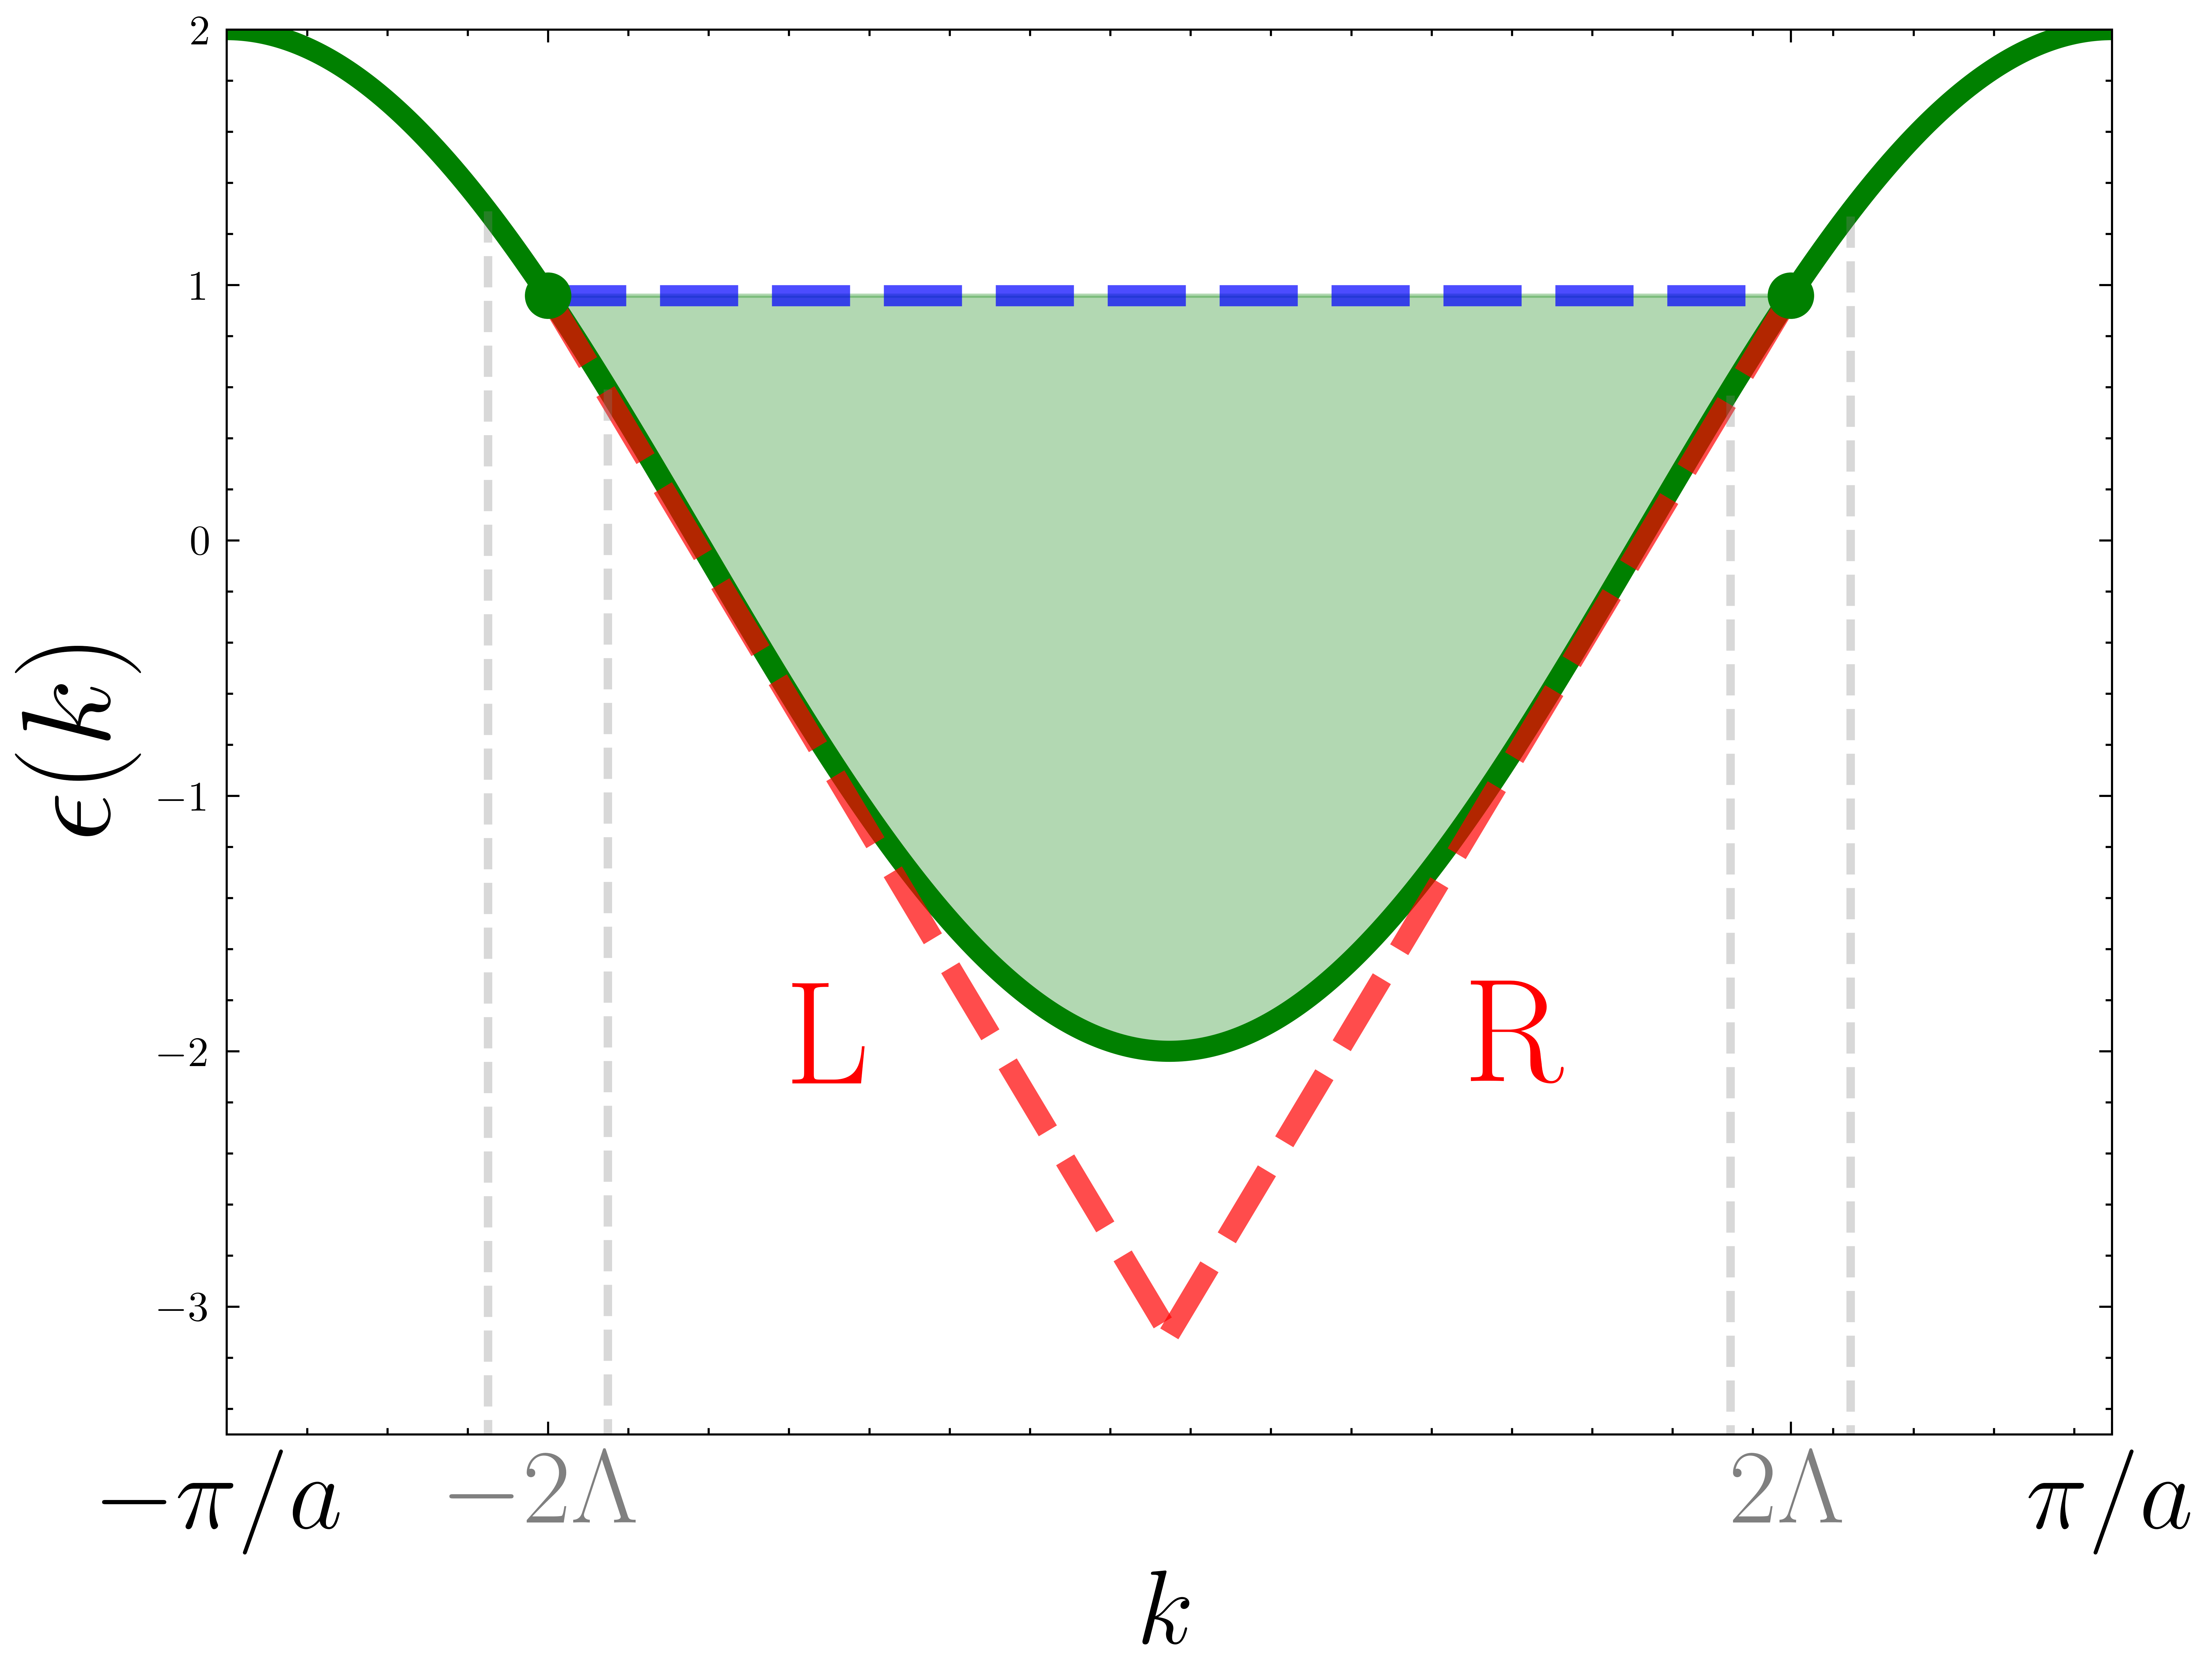
\includegraphics[scale=0.5]{Figures/Chapter 2/Grafica_Bosonization_Relation.png}
    \caption{Relacion de dispersión de un hamiltoniano de bosones libres.}
    \label{2_fig_bosonic_chirial}
\end{figure}
Es claro, que en la figura (\ref{2_fig_bosonic_chirial}) se ha pintado dos lineas que coinciden exactamente con el valor de la relación de dispersión para cuando observamos el sistema dentro de un intervalo $\Gamma$ especifico. Estas dos lineas nos permiten aproximar de manera exacta el sistema real descrito por el (\ref{2_H_free_bosons}) a un \textit{sistema efectivo} compuesto por dos sistemas lineales, que si bien no nos permiten describir el sistema real para todos los valores de momento, es exacto cuando nos encontramos dentro del intervalo mencionado. Esto indica que los operadores de destrucción y creación que diagonalizaban la relación de dispersión de la ecuación (\ref{2_H_free_bosons}) 
\begin{equation} \label{eq_a_momentum_operator}
\begin{aligned}
     \hat{b}(k)=\theta(k) \hat{\varphi}_{R}(k)+\theta(-k) \hat{\varphi}_{L}(k) \\
     \hat{b}^{\dagger}(k)=\theta(k) \hat{\varphi^{\dagger}}_{R}(k)+\theta(-k) \hat{\varphi^{\dagger}}_{L}(k)     
\end{aligned}   
\end{equation}
donde $\theta(k)$ es la función paso y $\hat{\varphi}_{R}(k)$, $\hat{\varphi}_{L}(k)$ son los campos de los operadores quiriales que describen \textit{efectivamente} el sistema. \\ \\
Entender el proceso anterior es esencial, como se puede apreciar en toda la literatura sobre bosonizacion [] siempre se empieza con esta imagen de linealización sobre el espectro de energía. Este es el concepto clave y que puede ser dificil al inicio de digerir.


\subsection{Single branch system.}
Ahora enfoquemonos en una sola rama del sistema que previamente hemos mencionado.


\subsection{Two branch system.}







\newpage
\section{Fields}
As mentioned at the beginning of this chapter, bosonization is a field theory, specifically a quantum field theory. To continue our discussion, it is important to define what we consider a free boson from the point of view of a quantum field theory. In principle, this must be done from a Lagrangian point of view. In the case of a massless bosonic field we have $\hat{\Phi}$:
\begin{equation} \label{2_2_1}
\hat{L_0}=\frac{1}{2} \int \mathrm{~d} x\left[\frac{1}{v}\left(\partial_t \hat{\Phi} (x)\right)^2-v\left(\partial_x  \hat{\Phi} (x)\right)^2\right],
\end{equation}
where $v$ is the Bose particle velocity. The Hamiltonian corresponding to the density would be
\begin{equation} \label{2_2_2}
    \hat{H}_0 = \frac{1}{2} v \big[ \frac{1}{v} (\hat{\Pi})^2
 -v(\partial \phi)^2 \big], 
\end{equation}
with $\hat{\Pi}$ being a conjugate field of $\phi$, the two fields obey the canonical commutation rules:
\begin{equation} \label{2_2_3}
    \big[ \hat{\Phi} (x), \hat{\Pi} (x) \big] = i \delta (x-x^{\prime}).
\end{equation}
The standard expansion for the fields $\hat{\phi}$ and $\hat{\Pi}$ in terms of their modes on an infinite line is given by:   
\begin{equation} \label{2_2_4}
    \hat{\Phi}(x, t)=\sum_{p \neq 0} \sqrt{\frac{1}{2 L|p|}}\left(e^{i\left(p x-|p| v_{E} t\right)} \hat{b}_{p}+\text { h.c. }\right),
\end{equation}
\begin{equation} \label{2_2_5}
   \hat{\Pi}(x, t)=-i \sum_{p \neq 0} \sqrt{\frac{|p|}{2 L}}\left(e^{i\left(p x-|p| v_{E} t\right)} \hat{b}_{p}-\text { h.c. }\right), 
\end{equation}
where $\hat{b}_{p}$ and $\hat{b}^{\dagger}_{p}$ are creation and destruction operators, and must obey the following commutation relation:
\begin{equation} \label{2_2_6}
    [\hat{b}_{p}, \hat{b}^{\dagger}_{p^{\prime}}] = 2\pi \delta (p-p^{\prime}),
\end{equation}
and allows the Hamiltonian to be expressed as follows:
\begin{equation} \label{2_2_7}
    \hat{H} = \int \frac{dk}{2\pi} \omega(k) \hat{b}_{k}^{\dagger} \hat{b}_{k}, 
\end{equation}
where $\omega (k) = v \abs{k}$ The ground (or vacuum) state $\ket{0}$ is destroyed by all operators $\hat{b} (k)$ and has zero energy by convection. It is worth noting and emphasizing that the previous Hamiltonian has a similar form to the one we have been working on from the beginning to visualize our formalism.\\ \\
Similarly, we can express the creation and destruction operators of the normal modes of the system in terms of the bosonic fields we have defined by adding the fields \ref{2_2_4} and \ref{2_2_5} and solving for each one we get:
\begin{equation} \label{2_2_8}
  \hat{b}_{p}  =\frac{-i}{\sqrt{2|p| L}} \int \mathrm{d} x e^{-i p x}\left(\operatorname{sgn}(p) \partial_{x} \hat{\Phi}-\hat{\Pi}\right)  \quad \quad   \hat{b}_{p}^{\dagger}  =\frac{i}{\sqrt{2|p| L}} \int \mathrm{d} x e^{i p x}\left(\operatorname{sgn}(p) \partial_{x} \hat{\Phi}-\hat{\Pi}\right) .
\end{equation}
It is important to define two additional fields, which allow us to work with the dynamics of the system:
\begin{equation} \label{2_2_9}
\hat{\theta}(x, t)=-\sum \frac{\operatorname{sgn}(p)}{\sqrt{2 L|p|}}\left(e^{i\left(p x-v_{E}|p| t\right)} \hat{b}_{p}+\text { h.c. }\right), 
\end{equation}
\begin{equation} \label{2_2_10}
\hat{\phi}_{\alpha}=\sum_{\alpha p>0} \sqrt{\frac{1}{2 L|p|}}\left(e^{i\left(p x-|p| v_{E} t\right)} \hat{b}_{p}+\text { h.c. }\right).
\end{equation}
\textcolor{myred}{Me gustaría añadir aqui unos parrafos hablando de la importancia y la necesidad de estos campos.}
\section{Bosonization Identity}
Now, in order to achieve functionally the bosonization identity with which we will work, we will follow the treatment made in [Ref: Giarmachi], we see that the main objective is to be able to have a bosonization identity that relates the creation and destruction operators of the original system in terms of bosonic fields that allow us to describe the dynamics of the system in a simpler way. To do this, we will change the point of view proposed in the previous sections, we will introduce a small new formalism that maintains the essence of the information, which is that: the current densities of the interactions that arise in the system are of a bosonic character.\\ \\
We can start with a one-dimensional boson (or fermion) system. The density operator for such a system is
\begin{equation} \label{B_I_eq_density}
    \hat{\rho}(x)=\sum_{i} \delta(x-x_{i}),
\end{equation}
where $x_{i}$ is the position of the i-th particle. Suppose that the position $R_{i}^{0}$ is called the "equilibrium position", this position would be the position occupied by the particle if the particles formed a perfect crystalline network, any displacement $u_{i}$ relative to this position is given by:
\begin{equation} \label{2_3_2}
    x_{i}=R_{i}^{0} + u_{i}.
\end{equation}
If we define $\rho_{0}$ as the mean density of the particle system, $d=\rho_{0}^{-1}$ is the distance between the particles. This would allow us to see that the equilibrium position of the i-th particle is:
\begin{equation}\label{2_3_3}
   R_{i}^{0}=di. 
\end{equation}
In order to deal more properly with the equation \eqref{B_I_eq_density}, we introduce the field $\Phi_{l}(x)$ in the same way as Haldane first did [Reference Haldane,1981b]. This field, which is a continuous function in position, takes the value $\hat{\Phi}_{l}(x_{i})=2\pi i$ when the particle is at the i-th position. This allows us to see another way of looking at the number of particles. This is a peculiarity of one-dimensional systems; unlike high-dimensional systems, we can always obtain the number of particles in a unique way, for example, by starting at $x= - \infty$ and contracting from left to right.\\ \\
\textcolor{myred}{Aquí iría otra grafica (2.3) extra que muestre el comportamiento del Campo $\hat{\phi}$ mencionado. } \\ \\
Using the following transformation rule for $\delta$ functions:
\begin{equation} \label{2_3_4}
    \delta(f(x)) = \sum \frac{1}{|f^{\prime}(x_{i})| \delta(x-x_{i})} ,
\end{equation}
we can rewrite the density \eqref{B_I_eq_density} as:
\begin{equation} \label{B_I_eq_rho_2}
    \begin{aligned} 
            \hat{\rho}(x) &=\sum_{i} \delta(x-x_{i}) \\
               &= \sum_{n} | \nabla \hat{ \Phi}_{l}(x)| \delta( \hat{\Phi}_{l}(x)-2\pi n). 
    \end{aligned}
\end{equation}
With the appropriate reference system, as we can see in figure (2.3:To be added), the field $ $ is always a function that increases with x, which allows us to leave aside the absolute value of \eqref{B_I_eq_rho_2}. Using the Posion summation formula, we can rewrite the equation as follows:
\begin{equation} \label{2_3_6}
    \hat{\rho} (x) = \frac{\nabla \hat{\Phi}_{l}(x)}{2\pi} \sum_{p} e^{ip \hat{\Phi}_{x}(x)},
\end{equation}
where $p$ is defined as an integer. It is convenient to define a field $\hat{\Phi}$ relative to the solution of the perfect crystal and introduce it as follows:
\begin{equation} \label{2_3_7}
    \hat{\Phi}_{l}(x) =2\pi \bar{\rho}_{0}x -2 \hat{\Phi}(x). 
\end{equation}
Thus, the density becomes:
\begin{equation} \label{B_I_rho_3}
    \hat{\rho}(x) = \big[\bar{\rho}_{0}-\frac{1}{\pi} \nabla \phi(x
)   \big] \sum_{p} e^{i2p(\pi \bar{\rho}_{0}x - \phi(x
))}.
\end{equation}
Since the density operator commutator commutes at two different locations in the lattice, we see that the fields $\phi_(x)$ commute with themselves. A special case of the equation \eqref{B_I_rho_3} occurs when the density is averaged over a distance large compared to the interparticle distance $d$, all oscillating terms disappear. This occurs when $p=0$, which is the density in this case:
\begin{equation} \label{2_3_8}
    \hat{\rho}(x) = \bar{\rho}_{0}-\frac{1}{\pi} \nabla \phi(x
).   
\end{equation}
This happens in the strongly correlated systems that we study and work on, we see that we can average over a large distance because it is comparable to the distance between particles. This means that these oscillating terms are important and necessary to adequately describe the dynamics of these systems. \\ \\
Following this line of thought we can go deeper by observing the behavior of a bosonic construction operator $\hat{b}^{\dagger}(x)$, we know that these operators can be written as follows:
\begin{equation}\label{B_I_eq_Identity}         
   \hat{b}^{\dagger} (x) = [\hat{\rho}(x)]^{1/2} e ^{-i\hat{\theta} (x)},
\end{equation}
where $\hat{\theta}(x)$ is some operator. It is known that the commutation relation between the creation and destruction operators is of bosonic character, which causes conditions to be imposed within the density operator of the system. As we will see below,
\begin{equation} \label{2_3_9}
    [\hat{b}(x), \hat{b}^{\dagger}(x^{\prime})] = \delta (x-x^{\prime}),
\end{equation}
substituting the information in the equation \ref{B_I_eq_Identity} we get the following expression:
\begin{equation}\label{B_I_eq_Long_Conmutator}
e^{+i \theta(x)}[\rho(x)]^{1 / 2}\left[\rho\left(x^{\prime}\right)\right]^{1 / 2} e^{-i \theta\left(x^{\prime}\right)}-\left[\rho\left(x^{\prime}\right)\right]^{1 / 2} e^{-i \theta\left(x^{\prime}\right)} e^{+i \theta(x)}[\rho(x)]^{1 / 2}
\end{equation}
%Colocar \hat equations.
Assuming reasonably that the field $\hat{\theta}$ commutes with the same $([\hat{\theta}(x),\hat{\theta}(x^{\prime})]=0)$, the commutator \ref{B_I_eq_Long_Commutator} is zero in the trivial case of $x\neq x^{\prime}$:
\begin{equation}  \label{2_3_10}
    [[\hat{\rho} (x)]^{1/2}, e^{-i \hat{\theta} (x)}]=0,
\end{equation}
which indicates that a sufficient condition satisfying the commutator in \eqref{2_3_9} is:
\begin{equation} \label{2_3_11}
    [\hat{\rho} (x), e ^{-i \hat{\theta} (x)}] = \delta (x-x^{\prime}) e^{-i \hat{\theta} (x)}.
\end{equation}
Now it is important to note that the contributions to the dynamics of our system are given by the density \eqref{2_3_8}, it is expected that both the fields $\hat{\Phi} (x)$ and $\hat{\theta} (x)$ vary slowly with respect to scales of the order of $\bar{\rho}_{0}^{-1}$. Assuming that the density behaves in this way, we get that:
\begin{equation} \label{2_3_12}
    \big[ \frac{1}{\pi} \nabla \hat{\Phi} (x),  \hat{\theta} (x^{\prime}) \big] = -i\delta (x-x^{\prime}),
\end{equation}
it is explicit that the above expression implies that the commutator of $\hat{\Phi}$ and $\hat{\theta}$ is of the form \ref{2_3_12}, as seen. Integrating the equation \ref{} by parts, it can be shown that
\begin{equation} \label{2_3_13}
    \pi \hat{\Pi} (x) = \nabla \hat{\theta} (x),
\end{equation}
where it can be seen that $\hat{\Pi}(x)$ is the canonical conjugate moment to $\hat{\Phi} (x)$. To obtain the single-particle operator, the equation \ref{B_I_rho_3} can be substituted in \ref{B_I_eq_Identity}, leading to:
\begin{equation} \label{2_3_14}
    \hat{b}_{B} = \sqrt{\bar{\rho} - \frac{1}{\pi} \nabla \hat{\Phi} (x)} \sum_{p} e^{i2p(\pi\bar{\rho}x - \hat{\Phi})} e^{-i\hat{\theta}}
\end{equation}
However, in this work we continue to work with the consideration presented in equation \ref{2_3_8}, which leads to our bosonization identity as follows:
\begin{equation} \label{2_3_15}
     \hat{b}_{B}^{\dagger} = \sqrt{\bar{\rho} - \frac{1}{\pi} \nabla \hat{\Phi} (x)}  e^{-i\hat{\theta}} \quad \quad  \hat{b}_{B} =  e^{i\hat{\theta}} \sqrt{\bar{\rho} - \frac{1}{\pi} \nabla \hat{\Phi} (x)}  
\end{equation}
The index $B$ emphasizes that we are representing a bosonic creation and destruction operator. The formulation for both destruction and construction operators is analogous. \\ \\
%----- Comentario---Punto de vista de la hidrodinamica.-------
\textcolor{myred}{También me gustaría hacer un comentario más desde el punto de vista de la hidrodinámica y de los sistemas de bosones unidimensionales, pero aún me tocaría refinar más el comentario, pero iría aqui, si se agrega.}


%\subsection{Hamiltoniano Giarmachi.}
%Mostrar el objetivo del hamiltoniano que se debe obtener a través de la bosonización.

\newpage

\section{Application: Bosons on a Lattice.}
Let us apply the formalism we have developed so far to the simplest but most illustrative case we can propose: one-dimensional bosons in a network. We begin by writing the Hamiltonian that describes the dynamics of the boson system in second quantization:
\begin{equation} \label{aqui1}
\hat{H}_{0}=-t \sum\left(\hat{a}_{i}^{\dagger} \hat{a}_{i+1}+\text { h.c. }\right).
\end{equation}
Reemplazando la información de podemos calcular $\hat{a}_{i}^{\dagger} \hat{a}_{i+1} $:
\begin{equation}
    \begin{aligned}
        \hat{a}_{i}^{\dagger} \hat{a}_{i+1} =\bar{\rho}\left(1+\frac{1}{2 \bar{\rho} \sqrt{K}} \partial_{x} \hat{\Phi} (x)\right) \exp \left(-i \sqrt{K} a \partial_{x} \hat{\theta} (x)\right)\left(1+\frac{1}{2 \bar{\rho} \sqrt{K}} \partial_{x} \hat{\Phi} (x)\right) \\
        \hat{a}_{i}^{\dagger} \hat{a}_{i+1}=\hat{\rho}(x)-\frac{a K}{2} \hat{\Pi}^{2} (x)+\frac{a}{4 K}\left(\partial_{x} \hat{\Phi} (x)\right)^{2}+\text { (imaginary part) }, 
    \end{aligned}
\end{equation}
where to get the previous result we worked in full fillin, $\bar{\rho}_{0}=a^{-1}$ and we kept the terms up to the first order in $a$. Thus, by adding the conjugate term of the Hamiltonian, we obtain the free Hamiltonian in its bosonized version:
\begin{equation} \label{eq_hamiltonian_asd}
\hat{H}_{0}=\frac{a t}{\sqrt{2}} \int \mathrm{d} x \hat{\Pi}^{2} (x)-\left(\partial_{x} \hat{\Phi} (x)\right)^{2}, 
\end{equation}
where we have used that $K=\frac{1}{\sqrt{2}}$. We see that this Hamiltonian differs by one sign from the version we found in the last section, namely, it is defined as a contribution of sums of quadratic fields. To see this difference, which is very important in this case, we can decompose the fields obtained in equation (\ref{2_2_4}) in terms of their normal modes using \ref{2_2_5}:%past equations of the fields
\begin{equation}
    \begin{aligned}
       \int \mathrm{d} x \hat{\Pi}^{2} (x) & =-\int \mathrm{d} x \sum_{p, q} \frac{\sqrt{|p q|}}{2 L}\left(e^{i x(p+q)} \hat{b}_{p} \hat{b}_{q}+e^{-i x(p+q)} \hat{b}_{p}^{\dagger} \hat{b}_{q}^{\dagger}-e^{i x(p-q)} \hat{b}_{p} \hat{b}_{q}^{\dagger}-e^{-i x(p-q)} \hat{b}_{p}^{\dagger} \hat{b}_{q}\right) \\
& =-\sum_{p} \frac{|p|}{2}\left(\hat{b}_{p} \hat{b}_{-p}+\hat{b}_{p}^{\dagger} \hat{b}_{-p}^{\dagger}-\hat{b}_{p} \hat{b}_{p}^{\dagger}-\hat{b}_{p}^{\dagger} \hat{b}_{p}\right),  
    \end{aligned}
\end{equation}
in the same way,
\footnotesize
\begin{equation}
    \begin{aligned}
        \int \mathrm{d} x\left(\partial_{x} \hat{\Phi} (x)\right)^{2}= & -\int \mathrm{d} x \sum_{p, q} \frac{\sqrt{|p q|}}{2 L} \operatorname{sgn}(p q)\left(e^{i x(p+q)} \hat{b}_{p} \hat{b}_{q}+e^{-i x(p+q)} \hat{b}_{p}^{\dagger} \hat{b}_{q}^{\dagger}\right.  \left.-e^{i x(p-q)} \hat{b}_{p} \hat{b}_{q}^{\dagger}-e^{-i x(p-q)} \hat{b}_{p}^{\dagger} \hat{b}_{q}\right) \\
= & \sum_{p} \frac{|p|}{2}\left(\hat{b}_{p} \hat{b}_{-p}+\hat{b}_{p}^{\dagger} \hat{b}_{-p}^{\dagger}+\hat{b}_{p} \hat{b}_{p}^{\dagger}+\hat{b}_{p}^{\dagger} \hat{b}_{p}\right),
    \end{aligned},
\end{equation}
\normalsize
%Al reescribir el Hamiltoniano en terminos de sus modos normales se obtiene:
%\begin{equation}
 %   s,
%\end{equation}
this ultimately leads us to the following conclusion:
\begin{equation}
\hat{H}_{0}=\frac{-a t}{\sqrt{2}} \sum_{p \neq 0}|p|\left(\hat{b}_{p} \hat{b}_{-p}+\hat{b}_{p}^{\dagger} \hat{b}_{-p}^{\dagger}\right). 
\end{equation}
At first glance, we might think that we are one Bogoliubov transformation away from diagonalizing the Hamiltonian, since we have quadratic contributions from the creation and destruction operators. However, when we perform the transformation:\\ \\
\textcolor{myred}{En la siguiente equación, en el futuro próximo, colocaré la información de la transformación de Bogoliuvov de manera explicita.}
\begin{equation}
    transformacionBV
\end{equation}
It is observed that there is no solution for the system, we have that $\alpha_{p}=0$ which leads to the complex angles defined $\varphi_{p}$ becoming $\beta_{p} \cosh{2\phi_{p}}$, which is not a solution. We see the first clear and concise indication that the system is unstable.\\ \\
We see that the dynamics of the bosons at low energy cannot be optimally described by bosonization when decomposed into their normal modes, nothing prevents the system from collapsing and forming a Bose-Einstein condensate. This can be clearly seen in what we mentioned at the beginning of this section, the negative term of the bosonized Hamiltonian [Ref],$-(\partial_{x} \hat{\Phi})^{2}$ represents an attractive force, which was expected for a system of free bosons. We can also observe that by performing the factorization process in the Hamiltonian [Ref.] we would find an imaginary Luttinger parameter, which would imply a breaking of the continuum limit[refe]. \\ \\
Now we know that a repulsive interaction between the bosons is needed to prevent them from collapsing, and that this interaction in turn causes the particles to inevitably collide with each other, creating the collective excitations that bosonization adequately describes. Does it make sense to consider a contact interaction within our particles? The answer is yes, in atomic physics a repulsive and contact interaction occurs as the limiting heat of s-wave scattering, and this simplification allows us to adequately and usefully describe low-energy particle collisions. In the context of our thesis goal, which is to describe ultracold bosons confined in an optical lattice, we see that these conditions are satisfied and allow this type of interaction. To do this, consider that in our approximation we have an interaction between two particles that are at the same point in space; at the same point in the lattice, so the interaction occurs when a site in the lattice is occupied by multiple bosons. With this in mind the two-body potential that we have to add to the Hamiltonian is of the form:
\begin{equation} \label{eq_21231}
    \hat{V} =\frac{g}{2} \sum_{i} \hat{b}^{\dagger}_{}\hat{b}^{}_{i}\hat{b}^{\dagger}_{i}\hat{b}^{}_{i},
\end{equation}
where the interaction strength $g$ is proportional to the scattering length of the system. We see that we apply the bosonization identity given by equation (\ref{2_3_15}) to equation (\ref{eq_21231}) and obtain directly its expression in terms of the bosonized fields
\begin{equation}
    \hat{V} = \frac{ag}{\sqrt{2}} \int dx \left( \hat{\Phi}\right)^{2},
\end{equation}
adding this term to (\ref{eq_hamiltonian_asd}), leads to having the complete term of the bosonized Hamiltonian:
\begin{equation} \label{hamiltonian2}
    \hat{H} = \frac{u}{\sqrt{2}} \int dx \left( \frac{1}{k}   \hat{\Pi}^{2} + K\left(\partial_{x} \hat{\Phi}\right)^{2} \right), 
\end{equation}
where $u = a \sqrt{t(g-t)} $ is the phase velocity of the excitations and $K = \sqrt{g/t -1}$ is the Luttinger parameter [Reference]. Which gives us a constraint within the system, as long as these values are real, bosonization will work.\\ \\
%---Text about it.

\subsection{Hard-Core Bosons.}
Hard-core bosons are particles that, although they are bosons (they are governed by Bose-Einstein statistics), have an additional restriction: they cannot occupy the same quantum state or physical space as another hard-core boson. In a way, this rule seems similar to the Pauli exclusion principle, which states that two fermions cannot occupy the same quantum state. Although both hard-core bosons and fermions cannot occupy the same quantum state, the wave function of a system of $N$ hard-core bosons does not follow the same antisymmetry rules as fermions. In the model we have described, especially in the case of the Hamiltonian (\ref{hamiltonian2}), we see that the parameters of the system can be changed to see microscopic properties of the system. Consider the case of interacting bosons in a lattice, when $g \rightarrow \infty$, the repulsion between pairs of bosons is so large that it does not allow two bosons to be in the same place in the lattice due to the large energy cost of multiple occupancy by particles.\\ \\
As mentioned above, this behavior of bosons is known from the Pauli exclusion principle, which allowed Girardeau to prove in 1960 that there is a direct mapping between repulsive bosons and free fermions [Ref:]. In particular, it was shown that the wave function describing both systems contains all the symmetry properties of bosons except for a spatially dependent phase. Writing this information in the second quantization formalism, one obtains that the relation between repulsive bosons and fermions is given by the Jordan-Wigner transformation:
\begin{equation} \label{aqui2}
    \hat{b}_{j} = e^{-i\pi t_{j}} \hat{c}_{j}, \quad \quad     \hat{b}^{\dagger}_{j} = e^{i\pi t_{j}} \hat{c}^{\dagger}_{j}, 
\end{equation}
where $\hat{c}_{j}$ are the fermionic operators and the bosonic operators remain $\hat{b}_{j}$, and $t_{j} = \sum_{k=0}^{j-1} \hat{n}_{k}$ is the string operator that guarantees the correct phase to satisfy the proper switching. We see that replacing the information from equation (\ref{aqui2}) into equation (\ref{aqui1}) gives the following Hamiltonian:
\begin{equation}
    \hat{H} = -t \sum \left( \hat{c}_{i}^{\dagger}\hat{c}_{i+1}^{} + \text{h.c}
 \right)  +\frac{g}{2} \sum \hat{c}_{i}^{\dagger}\hat{c}_{i}^{}\hat{c}_{i}^{\dagger}\hat{c}_{i}^{}.
\end{equation}
However, because double occupancy is prohibited due to the strong repulsion between particles at the same site, the second term vanishes, meaning it reduces to:
\begin{equation}
    \hat{H} = -t \sum \left( \hat{c}_{i}^{\dagger}\hat{c}_{i+1}^{} + \text{h.c}
 \right) 
\end{equation}
Showing that our main intuition was correct and that hard-core bosons are equivalent to free fermions [Reference]. The bosonization of these terms is similar to the bosonization we have applied previously, except that now our bosonization identity is for fermions [Appendix Tal.]. Thus the Hamiltonian describing the low-energy excitations of the system is:
\begin{equation}
    \hat{H} = \frac{at}{2} \int dx \left( \hat{\Pi}^{2} + \left(\partial_{x} \hat{\Phi}\right)^{2} \right)
\end{equation}
Showing that the Luttinger parameter for the hard-core boson case is $K=1$. This differs from the value found in equation \ref{hamiltonian2} where $K= \sqrt{g/t -1}$ for low energy scales, when $g \rightarrow \infty$ one would think that this term would diverge. However, we see that this is not the case.\\ \\
 \textcolor{myred}{Aún me falta leer un poco más en la literatura y justificar y hablar más sobre el anterior resultado.}


\subsection{Correlations.}
Once we have bosonized the one-dimensional hard-core bosons, we can calculate some correlation functions of the system. Mainly, we can calculate the density-density correlations, and the density matrix of the individual particles of the system.
\begin{equation}
\left\langle\hat{\rho}(x) \hat{\rho}(y)\right\rangle =   
\end{equation}

\begin{equation}
\left\langle\hat{c}^{\dagger}(x) \hat{c}(y)\right\rangle =   
\end{equation}

\textcolor{myred}{Hola profe, aquí quiero colocar el skim del paso a paso de los resultados de estas correlacionados, introducir como se calculan algunas de ellas, y si es posible la grafica de unas.}


\newpage
\begin{comment}
    
\section{Tabla Resumen.} 
Table \ref{table_summary_bosonization} below shows a brief bosonization dictionary, it summarized the main ingredients of the bosonization used in this chapter.
\begin{table}[h!]
  \captionsetup{justification=raggedright, singlelinecheck=false}
  \renewcommand{\arraystretch}{1.5} % Cambia el factor de interlineado a 1.5
  \caption{Bosonization Dictionary. The principals equations and definitions.}
  \begin{tabularx}{\textwidth}{l C r}
    \hline\hline
    Bosonic Behaviour: & $\left[ \hat{b}_{k \eta}^{\dagger} , \hat{b_{k^{\prime} \eta^\prime}} \right] = \delta_{kk^{\prime}} \delta_{\eta \eta^\prime}   \quad \eta = 1,...,M,$ &  \eqref{eq_prerequisites_1} \\
    Momentum Quantization: & $k = \frac{2\pi}{L} n_k \quad n_k \in \mathbb{N} $ & \eqref{eq_prerequisites_2} \\
    Momentum Quantization: & $\hat{H}_0 = \sum_k \frac{k^2}{2m} \hat{a}^{\dagger}(k) \hat{a}(k)$ & \eqref{eq_hamiltonian_free_bosons} \\
    Dispersion relation: &     $\epsilon(k) \approx \epsilon_{E} \pm\left(k \mp k_{E}\right) v_{E}$
 & \eqref{eq_dispersion_relation} \\
    Chirial system: &    $    \hat{a}(k)=\theta(k) \hat{\varphi}_{R}(k)+\theta(-k) \hat{\varphi}_{L}(k) $ & \eqref{eq_a_momentum_operator} \\
    Momentun: &    $        \begin{aligned}
            k_{E}+p_{R}, &\quad \text { if } k>0 \\
            -k_{E}+p_{L}, &\quad \text { if } k<0
        \end{aligned} $ & \eqref{eq_momentum_each_branch} \\
    Fourier operators: & $        \hat{a}(x)  =\frac{1}{\sqrt{L}} \sum_{k} e^{i k x} \hat{a}(k),
 $ & \eqref{eq_fuorier_definition_q} \\
    Fourier chirial field: & $\hat{\varphi}_{\alpha}(x)=\frac{1}{\sqrt{L}} \sum_{p} e^{i p x} \hat{\varphi}_{\alpha}(p)$ & \eqref{eq_fouerier_chrial_fields} \\
    : &    $ $ & \eqref{eq_dispersion_relation} \\
    
    \hline\hline
  \end{tabularx} \label{table_summary_bosonization}
\end{table}
\end{comment}



%\newpage
    
%You can see then that this chapter is self-contained and after we achieve the derivation of the Bosonic Identity the rest of our discussion will be a very brief application of it with bosons in a Lattice. This helps us think about the next chapter topic, which is the Bose-Hubbard model for spin-one particles. We begin with the necessary conditions before start thinking about bosonization, then, the next step is the formulation of the bosonization identity in terms of the bosonic field operators. After that, we'll look at the free bosons system. It's a well-known system that lets us test out the theory we've built and get a quick overview of some of the calculations we'll need to do on bosons systems.

\begin{comment}
   \section{Bosonization prerequisites}
%Comments
Before you start thinking about bosonization, it is 
 necessary to fulfill certain prerequisites. In this case, the idea is to reformulate a set of bosonic creation and annihilation operators with the canonical commutation relation:
\begin{align} \label{eq_prerequisites_1}
    & \left[ \hat{b}_{k \eta}^{\dagger} , \hat{b_{k^{\prime} \eta^\prime}} \right] = \delta_{kk^{\prime}} \delta_{\eta \eta^\prime}   &&  k \in [-\infty, \infty] && \eta = 1,...,M,
\end{align}
for a M species of bosons and a discrete, unbounded momentum (or wave number) index $k$ of the form
\begin{align} \label{eq_prerequisites_2}
    k = \frac{2\pi}{L} n_k &&   \text{with } n_k \in \mathbb{N}, 
\end{align}
L is the length of the system, specially, we need that the system satisfies the Born-Van Karman periodic boundary conditions[]. \\ \\
The periodicity of the system is going to be used here, when we consider a system of N bosons loaded in a 
%Dos condiciones de Felipe y el tma de Bloch.
The importance of the momentum index $k$ consist in the eigenergies of the system $\epsilon_k$ of the free and non-interacting system. The discrete and unbounded nature of $k$ is an essential prerequisite of the systematic derivation of the bosonization identity [].
 
\end{comment}













\section{Free Bosons}

Consider a system of $N$ spinless free bosons whose Hamiltonian is given by,
\begin{equation} \label{eq_hamiltonian_free_bosons}
    \hat{H}_0 = -2t \sum_k \cos{(lk)} \hat{a}^{\dagger}(k) \hat{a}(k)
\end{equation}
where $l$ is the longitude of the system and  $\hat{a}^{\dagger}(k) $ and $\hat{a}(k) $ refers to the creation and annihilation operators of the \textit{real system}. 

It has an explicit cosine dispersion relation $\epsilon_(k)=-2t\cos{(dk)}$ where $k$ is the quasi-momentum of the system and $t$ is an arbitrary constant that gives the amplitude of the hopping, we can define an interval of size $\Gamma$ around two specific points $\pm k_E$,  at low energies around which we desire to linearize the dispersion relation, the contributions to the physical properties of the system comes from the states close to $\pm k_E$ [], performing a Taylor expansion around $k_E$ reveals that the linear dispersion is
\begin{equation} \label{eq_dispersion_relation}
    \epsilon(k) \approx \epsilon_{E} \pm\left(k \mp k_{E}\right) \frac{\partial \epsilon (k)}{\partial k} \bigg|_{k=k_E} = \epsilon_{E} \pm\left(k \mp k_{E}\right) v_{E},
\end{equation}
where $v_E$ is given by $v_E =\frac{\partial}{\partial k} \epsilon (k_E) $

From the analogous of the Fermi surface, we can identify , at low energies, the contributions  to the dynamics of the system comes from the states close to $k_E$[].
\newpage


This is the case of interest, performing a T



according to the Solid State Theory [], we can define an analogous quantity to the Fermi Velocity in this system. In this case, $V_E$ is given by $v_E = \frac{\partial}{\partial k} \epsilon(k_E)$.The linearization process transforms the original system into a new system, a \textit{chirial system}.This system is is distinguished by two specific dispersion relations, one for each chiral wave function $\hat{a}$ , as illustrated in Figure \ref{fig_bosonic_chirial}.This linearization process occurs  in proximity to the energy level $K_E$, which implies that the mapping between the real and chiral systems is exact for dynamic contributions in this vicinity, it is.It can be demonstrated that the mapping between the real bosons $\hat{a}$ and the chiral particles can be placed in the 
\begin{equation} \label{eq_a_momentum_operator}
    \hat{a}(k)=\theta(k) \hat{\varphi}_{R}(k)+\theta(-k) \hat{\varphi}_{L}(k)
\end{equation}
The Heaviside step function, denoted by the symbol $\theta(k)$, is employed to partition the system into two particles, each with a positive moment of inertia, which move in the right branch. The opposite is true for the particles in the left branch. 
\begin{equation} \label{eq_momentum_each_branch}
    k=\left\{
        \begin{aligned}
            k_{E}+p_{R}, &\quad \text { if } k>0 \\
            -k_{E}+p_{L}, &\quad \text { if } k<0
        \end{aligned}
        \right.
\end{equation}
Replacing the information given by \eqref{eq_dispersion_relation}, \eqref{eq_a_momentum_operator} in \eqref{eq_hamiltonian_free_bosons}, and defining the chirial fields $\hat{\varphi}_{\alpha}(p)=\hat{\varphi}_{R / L}\left(\alpha k_{F}+p_{R / L}\right)$ with $\alpha \pm 1$ to represent the right and left branch respectively, we get
\begin{equation}
    \hat{H}_{0}=v_{E} \sum_{\alpha, p} \alpha p \hat{\varphi}_{\alpha}^{\dagger}(p) \hat{\varphi}_{\alpha}(p).
\end{equation}
As our next step, it is necessary to recognize that the operators described in equation \eqref{eq_a_momentum_operator} are not an appropriate description of the interactions of the system. The interactions of our system are located in space, so it is necessary to make a base change to our chiral operators that allows us to have their description in the position base. This is achieved by performing a Fourier series expansion in terms of the moment operator of the real system:
\begin{equation} \label{eq_fuorier_definition_q}
    \hat{a}(x)  =\frac{1}{\sqrt{L}} \sum_{k} e^{i k x} \hat{a}(k),
\end{equation}
Utilizing the aforementioned equation, we proceed to calculate the chirial operators in the position base:
\begin{equation} \label{eq_fourier_a_chirial}
    \begin{aligned}
\hat{a}(x) &  =\frac{1}{\sqrt{L}} \sum_{k} e^{i k x}\left(\theta(k) \hat{\varphi}_{R}(k)+\theta(-k) \hat{\varphi}_{L}(k)\right) \\
& =\frac{1}{\sqrt{L}} \sum_{p} e^{i k_{F} x} e^{i p x} \hat{\varphi}_{R}(k)+\frac{1}{\sqrt{L}} \sum_{p>} e^{-i k_{F} x} e^{i p x} \hat{\varphi}_{L}(k) \\
& =e^{i k_{F} x} \hat{\varphi}_{R}(x)+e^{-i k_{F} x} \hat{\varphi}_{L}(x),
\end{aligned}
\end{equation}
where we have used that position field also transform as follows
\begin{equation} \label{eq_fouerier_chrial_fields}
    \hat{\varphi}_{\alpha}(x)=\frac{1}{\sqrt{L}} \sum_{p} e^{i p x} \hat{\varphi}_{\alpha}(p).
\end{equation}

    
To proceed,


\begin{equation}
    \partial_{-\alpha} \hat{\varphi}_{\alpha}\left(x_{\alpha}\right)=0
\end{equation}






    
\textcolor{UVred}{\textbf{Preguntas/Dudas/Inquietudes:}}
Presento 4 dudas conceptuales profe, 2 de lo que ya he escrito y 2 que me han impedido seguir escribiendo.
\begin{itemize}
    \item La primera es sobre la ecuación (2.5) donde colocamos el operador $\hat{a}$ en terminos de los operadores de campo del sistema real. En este caso este operador $\hat{a}$ es bosonico. Pero lo que me confunde es que al realizar el mapeo en los sitemas quiriales estos se encuentran descritos por una línea, ya sea la linea de la izquierda o de la derecha. Cómo sabemos que al linealizar en estas ramas las particulas no se van al estado base (es decir, no se van hasta el estado menos infinito), debido a que son bosones cómo sabemos que al menos tendremos uno bosons distribuido a lo largo de la linea, es porque es un sistema 1D? Estuve viendo alguna literatura y se mencionar que se pueden tener interacciones de contacto en los bosones y llevaría a recobrar la física de Fermi-liquid. Sin embargo, sabiendo qué estamos en el caso de Luttinger liquids, cómo se podría justificar esto?
    \item  La segunda es sobre una sección que un comentario que también incluye felipe, especificamente el habla de esto:\\
""It might be tempting to rewrite the Hamiltonian of Eq. 2.6 in terms of the new position basis. In fact, the relationship between the temporal and spatial derivatives of the position operators given by Eq. 2.11 suggests the existence of a first-quantized operator $\hat{p}_{\alpha}$ with coordinate representation $-i \partial_{x} \delta\left(x-x^{\prime}\right)$. Consequently,
$$
\hat{H}_{0}=-i v_{F} \int \mathrm{d} x\left(\hat{\varphi}_{R}^{\dagger}(x) \partial_{x} \hat{\varphi}_{R}(x)-\hat{\varphi}_{L}^{\dagger}(x) \partial_{x} \hat{\varphi}_{L}(x)\right)
$$
From the literature we recognize a form of the Dirac Hamiltonian. There is, in fact, a close relationship between our low-energy theory and Dirac's relativistic formalism, and between systems with linear dispersions in general. However, bosonization deals with collective excitations so the microscopic formulation in terms of the individual chiral position operators is not adequate for our objective. In order to rewrite $\hat{H}_{0}$ with proper, well defined operators that represent collective degrees of freedom, let us address a surpisingly subtle nuance of a big aspect of bosonization."" \\ \\
Para este caso, cómo sabemos que podemos hacer el mismo comentario? Tenia entendido que este analogo se hacia debio al caracter fermionico de las particulas, pero ahora que estamos trabajando con bosones, podemos realizar la misma analogía? Por? Esto es importante porque de aquí es que se deduce que hay contribuciones cuadradticas de los operadores de corriente al cuadrado quiriales, entonces no sé cómo proceder con ello en las siguientes subsecciones.     
    \item  La tercera es respecto a los calculos de la siguientes subseciones, especialmente al calcular la forma del siguiente operador:
    

   \begin{align}
\hat{J}_{\alpha}^{2}(x) & =\lim _{\epsilon \rightarrow 0} \hat{J}_{\alpha}(x-\epsilon) \hat{J}_{\alpha}(x+\epsilon)  \\
& =\lim _{\epsilon \rightarrow 0}: \hat{\varphi}_{\alpha}^{\dagger}(x-\epsilon) \hat{\varphi}_{\alpha}(x-\epsilon):: \hat{\varphi}_{\alpha}^{\dagger}(x+\epsilon) \hat{\varphi}_{\alpha}(x+\epsilon):
\end{align} 

Aquí bo se usa point-sppliting cierto? debido a que ahora tenemos campos bosonicos dentro de nuestro sistema $\varphi$, seria realizar la multiplicación directa de ambos campos, utilizando claro, la relación de normal ordering que se presenta en la ecuación (2.18)?
\end{itemize}





\section{Normal Ordering}
    Now we might ask the following questions: What's the new behaviour of the new chirial system? it is physical possible? Primero estudiemos una rama del sistema chirial, sea sin perdida de generalidad la rama derecha como se presenta en la figura[ref]. Primero hay que notar que no hay un límite explícito del sistema, este proceso de linealización no lleva un sistema acotado, por lo que no podemos decir que hay un estado base? Esto esto posible físicamente? Vemos que la respuesta directa es no, el sistema real presenta un estado base como habiamos mencionado previamente. Sin embargo, vemos que el sistema chirial definido previamente presenta un comportamiento bosonico la ecuación (2.5) nos muetra que tenemos una combinación lineal de campos bosonicos, por lo que su comportamiento bosonico se mantiene en nuestro sistema linealizado. Esto llevaría a pensar que por las condiciones energ





    Literatura: Tesis de Felipe. + Fajardo + M. Peskin and D. Schroeder, “Interacting fields and feynman diagrams,” in Introduction to quantum field theory (Perseus Books, 1995), pp. 77–130.

\begin{equation}
: \hat{A}:=\hat{A}-\langle\hat{A}\rangle 
\end{equation}



\begin{align}
: \hat{A} \hat{A}^{\prime}:: \hat{B} \hat{B}^{\prime}: & =: \hat{A} \hat{A}^{\prime} \hat{B} \hat{B}^{\prime}: \nonumber \\
& +\langle\hat{A} \hat{B}\rangle: \hat{A}^{\prime} \hat{B}^{\prime}:+\left\langle\hat{A}^{\prime} \hat{B}^{\prime}\right\rangle: \hat{A} \hat{B}:+\left\langle\hat{A} \hat{B}^{\prime}\right\rangle: \hat{A}^{\prime} \hat{B}:+\left\langle\hat{A}^{\prime} \hat{B}\right\rangle: \hat{A} \hat{B}^{\prime}:  \tag{2.18}\\
& +\langle\hat{A} \hat{B}\rangle\left\langle\hat{A}^{\prime} \hat{B}^{\prime}\right\rangle+\left\langle\hat{A} \hat{B}^{\prime}\right\rangle\left\langle\hat{A}^{\prime} \hat{B}\right\rangle \nonumber
\end{align}



 




$$
\hat{\varphi}_{\alpha}(p, t)=\hat{\varphi}_{\alpha}(p, 0) e^{-\alpha i v_{E} p t}
$$

$$
\hat{\varphi}_{\alpha}(x, t)=\frac{1}{\sqrt{L}} \sum_{p} e^{-\alpha i p x_{\alpha}} \hat{\varphi}_{\alpha}(p, 0)
$$


$$
\hat{H}_{0}=-i v_{E} \int \mathrm{d} x\left(\hat{\varphi}_{R}^{\dagger}(x) \partial_{x} \hat{\varphi}_{R}(x)-\hat{\varphi}_{L}^{\dagger}(x) \partial_{x} \hat{\varphi}_{L}(x)\right)
$$














\section{Densities and Currents}

\begin{equation*}
\hat{J}_{\alpha}=: \hat{\varphi}_{\alpha}^{\dagger}(x) \hat{\varphi}_{\alpha}(x): \tag{2.14}
\end{equation*}



\begin{equation*}
\hat{\rho}(x)=\hat{J}_{R}(x)+\hat{J}_{L}(x), \quad \text { and } \quad \hat{J}(x)=v_{E}\left(\hat{J}_{R}(x)-\hat{J}_{L}(x)\right) \tag{2.15}
\end{equation*}



\begin{align*}
\partial_{t} \hat{\rho}+\partial_{x} \hat{J} & =0  \tag{2.16}\\
\partial_{x} \hat{\rho}+\frac{1}{v_{E}^{2}} \partial_{t} \hat{J} & =0
\end{align*}





\begin{align*}
\hat{J}_{\alpha}^{2}(x) & =\lim _{\epsilon \rightarrow 0} \hat{J}_{\alpha}(x-\epsilon) \hat{J}_{\alpha}(x+\epsilon)  \tag{2.17}\\
& =\lim _{\epsilon \rightarrow 0}: \hat{\varphi}_{\alpha}^{\dagger}(x-\epsilon) \hat{\varphi}_{\alpha}(x-\epsilon):: \hat{\varphi}_{\alpha}^{\dagger}(x+\epsilon) \hat{\varphi}_{\alpha}(x+\epsilon):
\end{align*}




\begin{align*}
\left\langle\hat{\varphi}_{\alpha}^{\dagger}(p) \hat{\varphi}_{\alpha}\left(p^{\prime}\right)\right\rangle & =\theta(-\alpha p) \delta_{p p^{\prime}}  \tag{2.19}\\
\left\langle\hat{\varphi}_{\alpha}(p) \hat{\varphi}_{\alpha}^{\dagger}\left(p^{\prime}\right)\right\rangle & =\theta(\alpha p) \delta_{p p^{\prime}}
\end{align*}



\begin{align*}
\left\langle\hat{\varphi}_{\alpha}^{\dagger}(x) \hat{\varphi}_{\alpha}(y)\right\rangle & =\frac{1}{L} \sum_{p p^{\prime}} e^{-i p x} e^{i p y}\left\langle\hat{\varphi}_{\alpha}^{\dagger}(p) \hat{\varphi}_{\alpha}\left(p^{\prime}\right)\right\rangle \\
& =\frac{1}{L} \sum_{p} e^{-i p(x-y)} \theta(-\alpha p)  \tag{2.20}\\
& =\frac{1}{2 \pi} \int \mathrm{d} p e^{-i p(x-y)} \theta(-\alpha p)
\end{align*}



\begin{align*}
\hat{J}_{\alpha}^{2}(x): & =\frac{-\alpha i}{2 \pi 2 \epsilon}\left(: \hat{\varphi}_{\alpha}(x-\epsilon) \hat{\varphi}_{\alpha}^{\dagger}(x+\epsilon):+: \hat{\varphi}_{\alpha}^{\dagger}(x-\epsilon) \hat{\varphi}_{\alpha}(x+\epsilon):\right) \\
& =\frac{-\alpha i}{2 \pi}\left(: \hat{\varphi}_{\alpha}^{\dagger}(x-\epsilon)\left(\frac{\hat{\varphi}_{\alpha}(x+\epsilon)-\hat{\varphi}_{\alpha}(x-\epsilon)}{2 \epsilon}\right):- \text { h.c }\right)  \tag{2.23}\\
& =\frac{-\alpha i}{2 \pi}\left(: \hat{\varphi}_{\alpha}^{\dagger}(x) \partial_{x} \hat{\varphi}_{\alpha}(x):- \text { h.c }\right)
\end{align*}

\begin{equation*}
\hat{H}_{0}=\pi v_{E} \int \mathrm{d} x\left(\hat{J}_{R}^{2}(x)+\hat{J}_{L}^{2}(x)\right) \tag{2.24}
\end{equation*}


\begin{equation*}
\left\langle\hat{\varphi}_{\alpha}^{\dagger}(x) \hat{\varphi}_{\alpha}(y)\right\rangle=\frac{1}{2 \pi} \int \mathrm{d} p e^{-\delta|p|} e^{-i p(x-y)} \theta(-\alpha p) \tag{2.25}
\end{equation*}


\begin{equation*}
\left\langle\hat{\varphi}_{\alpha}^{\dagger}(x) \hat{\varphi}_{\alpha}(y)\right\rangle=\frac{\alpha i}{2 \pi((x-y)+i \alpha \delta)} \tag{2.26}
\end{equation*}





\section{Particle - Hole fluctuations}


\begin{align*}
\hat{J}_{\alpha}(p) & =\frac{1}{\sqrt{L}} \sum_{q}: \hat{\varphi}_{\alpha}^{\dagger}(q-\alpha p) \hat{\varphi}_{\alpha}(q):  \tag{2.27}\\
\hat{J}_{\alpha}^{\dagger}(p) & =\hat{J}_{\alpha}(-p)
\end{align*}



\begin{equation*}
\hat{J}_{\alpha}(x)=\frac{1}{\sqrt{L}} \sum e^{\alpha i p x} \hat{J}_{\alpha}(p) \tag{2.28}
\end{equation*}


\begin{align*}
{\left[\hat{J}_{\alpha}(p), \hat{J}_{\alpha}^{\dagger}(p)\right] } & =\frac{1}{L} \sum_{q, q^{\prime}}\left[\hat{\varphi}_{\alpha}^{\dagger}(q-\alpha p) \hat{\varphi}_{\alpha}(q), \hat{\varphi}_{\alpha}^{\dagger}\left(q^{\prime}-\alpha p\right) \hat{\varphi}_{\alpha}\left(q^{\prime}\right)\right]  \tag{2.29}\\
& =\frac{1}{L} \sum_{q} \hat{\varphi}_{\alpha}^{\dagger}(q-\alpha p) \hat{\varphi}_{\alpha}(q-\alpha p)-\hat{\varphi}_{\alpha}^{\dagger}(q) \hat{\varphi}_{\alpha}(q)
\end{align*}



\begin{align*}
{\left[\hat{J}_{\alpha}(p), \hat{J}_{\alpha}^{\dagger}(p)\right] } & =\frac{1}{L} \sum_{q}: \hat{\varphi}_{\alpha}^{\dagger}(q-\alpha p) \hat{\varphi}_{\alpha}(q-\alpha p):-: \hat{\varphi}_{\alpha}^{\dagger}(q) \hat{\varphi}_{\alpha}(q):  \tag{2.30}\\
& +\left\langle\hat{\varphi}_{\alpha}^{\dagger}(q-\alpha p) \hat{\varphi}_{\alpha}(q-\alpha p)\right\rangle-\left\langle\hat{\varphi}_{\alpha}^{\dagger}(q) \hat{\varphi}_{\alpha}(q)\right\rangle \\
& =\frac{1}{L} \sum_{q} \theta(p-\alpha q)-\theta(-\alpha q) \\
& =\frac{p}{2 \pi}
\end{align*}



\begin{equation*}
\hat{b}(p)=A\left(\hat{J}_{R}(p) \theta(p) \pm \hat{J}_{L}(-p) \theta(-p)\right) \tag{2.31}
\end{equation*}



\begin{align*}
\hat{b}(p) & =-i \sqrt{\frac{2 \pi}{|p|}}\left(\hat{J}_{R}(p) \theta(p)-\hat{J}_{L}(-p) \theta(-p)\right)  \tag{2.32}\\
\hat{b}^{\dagger}(p) & =i \sqrt{\frac{2 \pi}{|p|}}\left(\hat{J}_{R}^{\dagger}(p) \theta(p)-\hat{J}_{L}^{\dagger}(-p) \theta(-p)\right)
\end{align*}


\begin{align*}
\hat{J}_{R}(p) & =i \sqrt{\frac{|p|}{2 \pi}}\left(\theta(p) \hat{b}_{p}-\theta(-p) \hat{b}_{-p}^{\dagger}\right)  \tag{2.33}\\
\hat{J}_{L}(p) & =-i \sqrt{\frac{|p|}{2 \pi}}\left(\theta(p) \hat{b}_{-p}-\theta(-p) \hat{b}_{p}^{\dagger}\right)
\end{align*}


\begin{align*}
\hat{H}_{0} & =\pi v_{E} \sum\left(\hat{J}_{R}(p) \hat{J}_{R}(-p)+\hat{J}_{L}(p) \hat{J}_{L}(-p)\right) \\
& =v_{E} \sum_{p \neq 0}|p| \hat{b}^{\dagger}(p) \hat{b}(p) \tag{2.37}
\end{align*}








%Books ese.




\chapter{Bose Hubbard Model (BHM)}
%%%%-----------------TEXTO:CAMBIARLO---------
The Bose-Hubbard model, a cornerstone in understanding many-body quantum systems, has profound applications in studying ultracold atoms in optical lattices. The connection between optical lattices and the Bose-Hubbard Hamiltonian provides insights into strongly correlated systems, especially when extended to spin-1 systems. This paper explores the relationship between these concepts in detail. \\ \\
\textcolor{myred}{Optical Lattices and Ultracold Atoms} \\ \\
Optical lattices are periodic potential structures formed by the interference of counter-propagating laser beams. These lattices create a periodic array of potential wells where ultracold atoms, typically bosons or fermions, can be trapped. These systems are tunable, allowing experimental control over key parameters such as lattice depth, atomic interactions, and hopping amplitude. This flexibility makes optical lattices ideal for simulating quantum many-body systems.

The dynamics of atoms in an optical lattice can be described by various models depending on the type of atoms and the interaction strengths. For bosonic atoms, the Bose-Hubbard model becomes particularly relevant as it captures the competition between kinetic energy and interactions, leading to a rich phase diagram including superfluid and Mott insulator phases. \\ \\
\textcolor{myred}{Bose-Hubbard Hamiltonian: Overview} \\ \\
The Bose-Hubbard Hamiltonian is commonly written as:

\begin{equation}
\hat{H} = -t \sum_{\langle i,j \rangle} (\hat{a}_i^\dagger \hat{a}_j + \hat{a}_j^\dagger \hat{a}_i) + \frac{U}{2} \sum_i \hat{n}_i (\hat{n}_i - 1) + \sum_i \epsilon_i \hat{n}_i
\end{equation}

where:
\begin{itemize}
    \item $t$ represents the hopping parameter between adjacent lattice sites,
    \item $\hat{a}_i^\dagger$ and $\hat{a}_i$ are the creation and annihilation operators for bosons at site $i$,
    \item $U$ denotes the on-site interaction energy,
    \item $\hat{n}_i$ is the number operator for site $i$,
    \item $\epsilon_i$ represents the local energy offset at site $i$.
\end{itemize}

This model effectively captures the physics of ultracold bosonic atoms in an optical lattice, allowing for the study of quantum phase transitions like the superfluid-to-Mott insulator transition. \\ \\
\textcolor{myred}{Spin-1 Systems and the Extended Bose-Hubbard Model}\\ \\


In a spin-1 system, the Bose-Hubbard model becomes more complex as the atoms can occupy multiple spin states, introducing additional degrees of freedom. The spin-1 variant of the Bose-Hubbard model incorporates spin-exchange interactions and can be written as:

\begin{equation}
\hat{H} = -t \sum_{\langle i,j \rangle} \sum_{m_s} (\hat{a}_{i,m_s}^\dagger \hat{a}_{j,m_s} + h.c.) + \frac{U_0}{2} \sum_{i} \hat{n}_i (\hat{n}_i - 1) + \frac{U_2}{2} \sum_i \left( \vec{S}_i^2 - 2 \hat{n}_i \right)
\end{equation}

where:
\begin{itemize}
    \item $U_0$ is the spin-independent interaction term,
    \item $U_2$ is the spin-dependent interaction term,
    \item $\vec{S}_i$ represents the total spin operator at site $i$,
    \item $\hat{a}_{i,m_s}$ denotes the annihilation operator for a boson with spin $m_s$ at site $i$.
\end{itemize}

This Hamiltonian describes the interplay between on-site interactions, hopping between lattice sites, and spin-dependent interactions. In the case of spin-1 bosons such as Sodium-23 or Rubidium-87 atoms, spin-dependent interactions lead to phenomena like spin nematicity, spinor condensates, and magnetization dynamics.\\ \\
\textcolor{myred}{Phases of Spin-1 Bose-Hubbard Model}\\ \\
%\subsection{Mott Insulator Phase}
In the Mott insulator phase, each lattice site is filled with a fixed number of atoms due to strong on-site interactions. For spin-1 atoms, this phase exhibits different magnetic orderings depending on the interaction strengths $U_0$ and $U_2$. The ground state can be either ferromagnetic (aligned spins) or anti-ferromagnetic (opposite spins) based on the sign of the spin-exchange term.

%\subsection{Superfluid Phase}

In the superfluid phase, atoms are delocalized across the lattice, and long-range coherence is established. The spinor nature of the atoms introduces additional complexity in this phase, where spin-mixing dynamics and magnetization properties play crucial roles.

%\subsection{Spinor Condensates}

Spin-1 systems can also form spinor Bose-Einstein condensates (BECs), which exhibit macroscopic quantum phenomena. Depending on the interaction parameters, these condensates can show polar, ferromagnetic, or nematic phases, characterized by different spin alignments.\\ \\
\textcolor{myred}{Experimental Realizations}\\ \\
Experiments with ultracold atoms in optical lattices have successfully implemented the Bose-Hubbard model for both scalar and spinor systems. Spin-1 atoms such as Rubidium-87 (Rb-87) or Sodium-23 (Na-23) are commonly used to explore spinor physics. By adjusting the lattice depth, interaction strength, and external magnetic fields, researchers have observed quantum phase transitions and spin-ordering phenomena in these systems.

One notable example is the observation of a Mott insulator phase with spin-1 bosons in a three-dimensional optical lattice, where researchers could probe spin correlations and spin-dependent dynamics using advanced techniques like quantum gas microscopy.\\ \\
\textcolor{myred}{Theoretical Extensions and Applications}
The spin-1 Bose-Hubbard model serves as a foundation for exploring more exotic quantum phenomena. The interplay of spin and particle interactions leads to a variety of interesting phases, including:
\begin{itemize}
    \item \textbf{Spin-Nematic Phases:} These phases lack magnetic order but possess a quadrupolar order, leading to unique properties in spinor systems.
    \item \textbf{Magnetization Dynamics:} The spin-1 system allows the study of magnetization and spin-mixing dynamics, which are essential for understanding magnetic ordering in quantum systems.
\end{itemize}

The model also provides a framework for exploring quantum magnetism in optical lattices, where spin-dependent interactions can be tuned to mimic magnetic systems with controlled parameters. \\ \\
\textcolor{myred}{Conclusiones}\\
%\section{Conclusion}
The relationship between optical lattices and the spin-1 Bose-Hubbard Hamiltonian opens up rich avenues for exploring quantum many-body systems, spinor condensates, and quantum magnetism. Optical lattices provide a highly controllable experimental platform, while the spin-1 Bose-Hubbard model captures the essential physics of interacting spinor bosons. The study of these systems is crucial for understanding complex quantum phenomena such as superfluidity, magnetism, and quantum phase transitions.

%\section*{References}

\begin{enumerate}
    \item Bloch, I., Dalibard, J., \& Zwerger, W. (2008). Many-body physics with ultracold gases. \textit{Reviews of Modern Physics}, 80(3), 885-964.
    \item Lewenstein, M., Sanpera, A., Ahufinger, V. (2012). \textit{Ultracold Atoms in Optical Lattices: Simulating Quantum Many-Body Systems}. Oxford University Press.
    \item Greiner, M., Mandel, O., Esslinger, T., Hänsch, T. W., \& Bloch, I. (2002). Quantum phase transition from a superfluid to a Mott insulator in a gas of ultracold atoms. \textit{Nature}, 415(6867), 39-44.
    \item Demler, E., \& Zhou, F. (2002). Spinor Bosonic Atoms in Optical Lattices: Symmetry Breaking and Fractionalization. \textit{Physical Review Letters}, 88(16), 163001.
    \item Auerbach, A. (1998). \textit{Interacting Electrons and Quantum Magnetism}. Springer.
\end{enumerate}
%%%%------------------------------%%%
\newpage
\section{Bosonization.}
Recobrando la información esencial de la mini introducción, es que nuestro Hamiltonino, al estar bajo la influencia de un potencial químico y campo de zeman lineal se puede ver de la siguiente manera:
\begin{equation}
    \hat{H}=\overbrace{-t \sum_{\langle i, j\rangle, \sigma}\left(\hat{b}_{i, \sigma}^{\dagger} \hat{b}_{j, \sigma}+\text { h.c. }\right)}^{\text {Hopping}} \underbrace{+\hat{H}_I}_{\text {Interaction}} \overbrace{-\mu \sum_i \hat{n}_{i, \sigma}}^{\text {Chemical Potential }}+\overbrace{q \sum_{i, \sigma} \sigma \hat{n}_{i, \sigma}}^{\text {Zeeman Field}} \text{,}
\end{equation}
donde el termino de interacción tiene la siguiente forma:
\footnotesize 
\begin{align}
    \hat{H}_{I} = &\sum_i \Bigg[ \underbrace{\frac{g_2}{2} \left( \hat{b}_{1}^{\dagger}\hat{b}_{1}^{\dagger} \hat{b}_{1}^{} \hat{b}_{1}^{} 
    + \hat{b}_{-1}^{\dagger}\hat{b}_{-1}^{\dagger} \hat{b}_{-1}^{} \hat{b}_{-1}^{} 
    + 2\hat{b}_{1}^{\dagger}\hat{b}_{0}^{\dagger} \hat{b}_{1}^{} \hat{b}_{0}^{}  
    + 2\hat{b}_{-1}^{\dagger}\hat{b}_{0}^{\dagger} \hat{b}_{-1}^{} \hat{b}_{0}^{} \right) 
    + \frac{2g_{2} + g_{0}}{6} \hat{b}_{0}^{\dagger}\hat{b}_{0}^{\dagger} \hat{b}_{0}^{} \hat{b}_{0}^{}+\frac{g_{2} + 2g_{0}}{3} + 2\hat{b}_{1}^{\dagger}\hat{b}_{-1}^{\dagger} \hat{b}_{-1}^{} \hat{b}_{1}^{} }_{\text {Spin Preserving Collision}}  \nonumber \\
 +&\underbrace{\frac{g_{2}-g_{0}}{3} \left( \hat{b}_{-1}^{\dagger}\hat{b}_{1}^{\dagger} \hat{b}_{0}^{} \hat{b}_{0}^{} + \hat{b}_{0}^{\dagger}\hat{b}_{0}^{\dagger} \hat{b}_{1}^{} \hat{b}_{-1}^{}\right)}_{\text {Spin Changing Collision}} 
    \Bigg]_{i}.
\end{align}
\normalsize
Antes de iniciar el proceso de bosonización es importante identificar dos cosas. La primera es ver que tenemos operadores de creación y destrucción para cada proyección mágnetica de spin de las partículas. Este comportamiento nos da indiciones que podemos llegar a tener una identidad de bosonización diferente para cada una de estas proyecciones mágneticas. Sin embargo, tiene algún sentido físico pensar que el sistema se comporta así? Veamos que este sí es el caso, al realizar una transformada de Fourier a todo nuestro Hamiltonian \eqref{} exeptuando el termino de interacción:
\begin{equation}
    \hat{H}=\overbrace{-t \sum_{\langle i, j\rangle, \sigma}\left(\hat{b}_{i, \sigma}^{\dagger} \hat{b}_{j, \sigma}+\text { h.c. }\right)}^{\text {Hopping}}  \overbrace{-\mu \sum_i \hat{n}_{i, \sigma}}^{\text {Chemical Potential }}+\overbrace{q \sum_{i, \sigma} \sigma \hat{n}_{i, \sigma}}^{\text {Zeeman Field}} \text{,}
\end{equation}
aplicamos la siguiente transformada de fourier a nuestro sistema:
\begin{equation}
    \hat{b_j} = \frac{1}{\sqrt{L}} \sum_{k=1}^{n} e^{-2\pi i jk/n}  \hat{b}_{k} \quad \quad \hat{b_j}^{\dagger} = \frac{1}{\sqrt{L}} \sum_{k=1}^{n} e^{2\pi i jk/n} \hat{b}_{k}^{\dagger}
\end{equation}
donde $\hat{b_j}$ y $\hat{b_j}^{\dagger}$ son operadores de construcción y destrucción en el espacio de momento [Organizar esto, estamos pasando de espacio a momento.]. Volviendo a la equación \eqref{}, vemos que se puede descomponer en dos partes, una que contiene la información del termino de salto y otra que contiene tanto la información del potencial químico como del campo lineal de Zeeman:
\begin{equation}
    \hat{H}=\overbrace{-t \sum_{\langle i, j\rangle, \sigma}\left(\hat{b}_{i, \sigma}^{\dagger} \hat{b}_{j, \sigma}+\text { h.c. }\right)}^{\text {Hopping}}  \overbrace{-\mu \sum_i \hat{n}_{i, \sigma}}^{\text {Chemical Potential }}+\overbrace{q \sum_{i, \sigma} \sigma \hat{n}_{i, \sigma}}^{\text {Zeeman Field}} \text{,}
\end{equation}
Así, aplicando la trnasformadad de Fouierdad dada por la equación \eqref{} a la eqcuación \eqref{} se obtiene para el primer termino:



\begin{align}
     \hat{H} = -t \sum_{<i,j>} \left( \hat{b}_{i,\sigma}^{\dagger}\hat{b}_{j,\sigma}^{} + \hat{b}_{j,\sigma}^{\dagger} \hat{b}_{i,\sigma}^{} \right) \\
     = \sum_asdas = otro por poner = \sum_{k} \left( -2t \cos{(\frac{2\pi}{L} k)} + (B \sigma - \mu) \right) \hat{b}_{k,\sigma}^{\dagger} \hat{b}_{k,\sigma}^{}  \\
      sss
\end{align}
A su vez, realizando la 


 \begin{align}
    \hat{H} = \sum_{k} \left( -2t \cos{(\frac{2\pi}{L} k)} + (B - \mu) \right) \hat{b}_{k,1}^{\dagger} \hat{b}_{k,1}^{} \nonumber \\
    +\sum_{k} \left( -2t \cos{(\frac{2\pi}{L} k)}  - \mu \right) \hat{b}_{k,0}^{\dagger} \hat{b}_{k,0}^{} \\
    + \sum_{k} \left( -2t \cos{(\frac{2\pi}{L} k)} - (B + \mu) \right) \hat{b}_{k,-1}^{\dagger} \hat{b}_{k,-1}^{}   \nonumber
 \end{align}
Vemos que se obtiene de manera explícita una relación cosenoidal para cada uno de los operadores de creación y destrucción según su proyección magnetica. Se observa que algunos partículas son beneficiadas o perjudicadas en terminos energeticos con la presencia de un campo magnético. Esto es



Al graficar las diferentes proyecciones magnéticas, observamos que podemos realzar un proceso de bosonización en cada una de ellas [Fig Tal] [Fig 3: 1: Una sola proyección magnetica, 2: Las tres, 4: Esquema de los niveles de energía.]\\ \\

Lo que verdaderamente cambia dentro el proceso formal de la bosonización que hemos descrito en el capítulo anterior es la ecuación \eqref{} que habla de las densidades medias, vemos que ahora no se tiene una única densidad media para todas las partículas, sino, que esta depende de la proyección magnética de las partículas. Es claro que las densidades medias de las proyecciones magnéticas difieren entre si en presencia de un campo magnético lineal externo. Esto nos lleva a concluir, colocando la información mencionada en la \eqref{} que la identidad de bosonización toma la siguiente forma:
\begin{align}
    \hat{\rho} = \bar{\rho}_{0} + \frac{\partial_{x} \hat{\Phi}_{\sigma}}{\sqrt{k}} \\
    \hat{b}_{\sigma}^{\dagger} (x) = \sqrt{ \bar{\rho}_{0} + \frac{\partial_{x} \hat{\Phi}_{\sigma}}{\sqrt{k}}} e^{i \sqrt{k} \hat{\theta_{\sigma}}} \\
    \hat{b}_{\sigma}^{} (x) = e^{-i \sqrt{k} \hat{\theta_{\sigma}}} \sqrt{ \bar{\rho}_{0} + \frac{\partial_{x} \hat{\Phi}_{\sigma}}{\sqrt{k}}} 
\end{align}
Colocando esta información en términos de colores y siendo congruentes con la ecuación \eqref{} se tiene que:


\begin{equation}
\begin{aligned}
    \textcolor{mygreen}{\hat{\rho}_{1} = \bar{\rho}_{1} + \frac{\partial_{x} \hat{\Phi}_{1}}{\sqrt{k}}} \quad \quad & \textcolor{mygreen}{\hat{b}_{1}^{\dagger} (x) = \sqrt{ \bar{\rho}_{1} + \frac{\partial_{x} \hat{\Phi}_{1}}{\sqrt{k}}} e^{i \sqrt{k} \hat{\theta_{1}}}} \quad \quad & \textcolor{mygreen}{\hat{b}_{1}^{} (x) = e^{-i \sqrt{k} \hat{\theta_{1}}} \sqrt{ \bar{\rho}_{1} + \frac{\partial_{x} \hat{\Phi}_{1}}{\sqrt{k}}} } \quad 
\end{aligned}
\end{equation}


\begin{equation}
\begin{aligned}
    \textcolor{myblue}{\hat{\rho}_{0} = \bar{\rho}_{0} + \frac{\partial_{x} \hat{\Phi}_{0}}{\sqrt{k}}} \quad \quad & \textcolor{myblue}{\hat{b}_{0}^{\dagger} (x) = \sqrt{ \bar{\rho}_{0} + \frac{\partial_{x} \hat{\Phi}_{0}}{\sqrt{k}}} e^{i \sqrt{k} \hat{\theta_{0}}}} \quad \quad & \textcolor{myblue}{\hat{b}_{0}^{} (x) = e^{-i \sqrt{k} \hat{\theta_{0}}} \sqrt{ \bar{\rho}_{0} + \frac{\partial_{x} \hat{\Phi}_{0}}{\sqrt{k}}} } \quad 
\end{aligned}
\end{equation}

\footnotesize
\begin{equation}
\begin{aligned}
    \textcolor{myred}{\hat{\rho}_{-1} = \bar{\rho}_{-1} + \frac{\partial_{x} \hat{\Phi}_{-1}}{\sqrt{k}}} \quad \quad &  \textcolor{myred}{\hat{b}_{-1}^{\dagger} (x) = \sqrt{ \bar{\rho}_{-1} + \frac{\partial_{x} \hat{\Phi}_{-1}}{\sqrt{k}}} e^{i \sqrt{k} \hat{\theta_{-1}}}} \quad \quad  & \textcolor{myred}{\hat{b}_{-1}^{} (x) = e^{-i \sqrt{k} \hat{\theta_{-1}}} \sqrt{ \bar{\rho}_{-1} + \frac{\partial_{x} \hat{\Phi}_{-1}}{\sqrt{k}}} } 
\end{aligned}
\end{equation}\\ \\
\normalsize
La segunda cosa que es importante identificar se refiere a la ecuación \eqref{} que nos indica el hamiltoniano de interacción, donde cada uno de los terminos se puede escribir de una manera general y conveniente para el proceso de bosonización:
\footnotesize 
\begin{align}
    \hat{H}_{I} = &\sum_i \Bigg[ \underbrace{\frac{g_2}{2} \left( \hat{b}_{1}^{\dagger}\hat{b}_{1}^{\dagger} \hat{b}_{1}^{} \hat{b}_{1}^{} 
    + \hat{b}_{-1}^{\dagger}\hat{b}_{-1}^{\dagger} \hat{b}_{-1}^{} \hat{b}_{-1}^{} 
    + 2\hat{b}_{1}^{\dagger}\hat{b}_{0}^{\dagger} \hat{b}_{1}^{} \hat{b}_{0}^{}  
    + 2\hat{b}_{-1}^{\dagger}\hat{b}_{0}^{\dagger} \hat{b}_{-1}^{} \hat{b}_{0}^{} \right) 
    + \frac{2g_{2} + g_{0}}{6} \hat{b}_{0}^{\dagger}\hat{b}_{0}^{\dagger} \hat{b}_{0}^{} \hat{b}_{0}^{}+\frac{g_{2} + 2g_{0}}{3} + 2\hat{b}_{1}^{\dagger}\hat{b}_{-1}^{\dagger} \hat{b}_{-1}^{} \hat{b}_{1}^{} }_{\text {Spin Preserving Collision}}  \nonumber \\
 +&\underbrace{\frac{g_{2}-g_{0}}{3} \left( \hat{b}_{-1}^{\dagger}\hat{b}_{1}^{\dagger} \hat{b}_{0}^{} \hat{b}_{0}^{} + \hat{b}_{0}^{\dagger}\hat{b}_{0}^{\dagger} \hat{b}_{1}^{} \hat{b}_{-1}^{}\right)}_{\text {Spin Changing Collision}} 
    \Bigg]_{i}.
\end{align}
\normalsize
Vemos que el proceso de bosonización del termino de interacción se encuentra completado al bosonizar los terminos $ 1$, $2$, $3$ y $4$.

Ahora estamos listos para iniciar el proceso de bosonización de nuestro hamiltoniano de estudio. Para ello, tenemos presente las relaciones dadas  en la \eqref{}, las relaciones de conmutación que se encuentran en \eqref{} y la aproximación a primer orden mostrada en \eqref{}. Primero realizaremos la bosonización del hamiltoniano \eqref{} iniciando por los terminos que no pertenecer a la interacción:
\subsection{Bosonization: Kinetic term:}
Enfocandonos en este termino que es de la forma 
\begin{equation}
\hat{H} = -t \sum_{<i,j>} \left( \hat{b}_{i,\sigma}^{\dagger}\hat{b}_{j,\sigma}^{} + \hat{b}_{j,\sigma}^{\dagger} \hat{b}_{i,\sigma}^{} \right)
\end{equation}
Al aplicar el proceso de bosonización obtenemos:
\begin{align}    \hat{b}_{i,\sigma}^{\dagger}\hat{b}_{j,\sigma}^{} = &\sqrt{\bar{\rho_{\sigma}}} \left( 1+\frac{\partial_{x} \hat{\Phi}_{\sigma}} {2\bar{\rho}_{\sigma} \sqrt{k}} \right) e^{i \sqrt{k} \hat{\theta_{\sigma}}} \sqrt{\bar{\rho_{\sigma}}} e^{-i \sqrt{k} \hat{\theta_{\sigma}}} \left( 1+\frac{\partial_{x} \hat{\Phi}_{\sigma}} {2\bar{\rho}_{\sigma} \sqrt{k}} \right) \\
    &=\bar{\rho_{\sigma}} \left( 1+\frac{\partial_{x} \hat{\Phi}_{\sigma}} {2\bar{\rho}_{\sigma} \sqrt{k}} \right) e^{-i\sqrt{k} (\hat{\theta}_{\sigma}(x+a) - \hat{\theta}_{\sigma} (x))} \left( 1+\frac{\partial_{x} \hat{\Phi}_{\sigma}} {2\bar{\rho}_{\sigma} \sqrt{k}} \right)\\
    &=\bar{\rho_{\sigma}} \left( 1+\frac{\partial_{x} \hat{\Phi}_{\sigma}} {2\bar{\rho}_{\sigma} \sqrt{k}} \right) e^{-i\sqrt{k}a \partial_{x}\hat{\theta}_{\sigma}}\left( 1+\frac{\partial_{x} \hat{\Phi}_{\sigma}} {2\bar{\rho}_{\sigma} \sqrt{k}} \right)\\
    &= \left( \bar{\rho_{\sigma}}+\frac{\partial_{x} \hat{\Phi}_{\sigma}} {2 \sqrt{k}} \right) e^{-i\sqrt{k}a \partial_{x}\hat{\theta}_{\sigma}}\left( 1+\frac{\partial_{x} \hat{\Phi}_{\sigma}} {2\bar{\rho}_{\sigma} \sqrt{k}} \right) \\
    &=\left( \bar{\rho_{\sigma}}+\frac{\partial_{x} \hat{\Phi}_{\sigma}} {2 \sqrt{k}} \right) \left( 1-i\sqrt{k}a \hat{\Phi} - \frac{ka^2 \hat{\Phi}^2}{2} \right) \left( 1+\frac{\partial_{x} \hat{\Phi}_{\sigma}} {2\bar{\rho}_{\sigma} \sqrt{k}} \right) \\
    &= \left( \bar{\rho_{\sigma}}+\frac{\partial_{x} \hat{\Phi}_{\sigma}} {2 \sqrt{k}} \right) \left( ... \right)
\end{align}
DE manera analoga se realiza el calculo de $\hat{b}_{j,\sigma}^{\dagger} \hat{b}_{i,\sigma}^{} $, lo que lleva como resultado a:
\begin{equation}
    \hat{H} = -t \sum_{<i,j>} \left( \hat{b}_{i,\sigma}^{\dagger}\hat{b}_{j,\sigma}^{} + \hat{b}_{j,\sigma}^{\dagger} \hat{b}_{i,\sigma}^{} \right) =  \sum_{\sigma} -2t \hat{\rho}_{\sigma} (x) + t \bar{\rho}_{\sigma} k a^{2} \hat{\Phi}^{2} - t \frac{(\partial_{x} \hat{\Phi}_{\sigma} )^2}{2 \bar{\rho}_{\sigma} k}
\end{equation}
Lo que quiere decir que es igual a:
\begin{equation}
       \hat{H} = -t \sum_{<i,j>} \left( \hat{b}_{i,\sigma}^{\dagger}\hat{b}_{j,\sigma}^{} + \hat{b}_{j,\sigma}^{\dagger} \hat{b}_{i,\sigma}^{} \right) =\sum_{\sigma} t   \int  dx\left(\bar{\rho}_{\sigma} k a^{2} \hat{\Pi}^{2} - t \frac{(\partial_{x} \hat{\Phi}_{\sigma} )^2}{2 \bar{\rho}_{\sigma} k}  \right)
\end{equation}
Vemos que este término se puede escribir de manera matricial de la siguiente forma:\\ 
%[ESCRIBIR FORMA MATRICIAL]



\subsection{bosonization: Chemical Potential and Linear Magnetic Field} \textbf{Bosonization of the Zeeman/Chemical term}
Falta añadir el proceso pero:
\begin{equation}
    \hat{H}_{B,\mu}= \overbrace{-\mu \sum_i \hat{n}_{i, \sigma}}^{\text {Potencial químico }}+\underbrace{q \sum_{i, \sigma} \sigma \hat{n}_{i, \sigma}}_{\text {Campo de Zeeman}}
\end{equation}
\begin{equation}
    \hat{H}_{B,\mu}=\int dx \left( -\mu \frac{\sqrt{3} \partial_{x}\hat{\Phi}_c}{\sqrt{k}}  + B \frac{\sqrt{2} \partial_{x}\hat{\Phi}_s}{\sqrt{k}} \right)
\end{equation}




\subsection{bosonization of the interacction term}
\subsubsection{Interaction Term: Spin Preserving Collisions.}


\subsubsection{Interaction Term: Spin Changing Collisions.}

\section{Still working on the Hamiltonian - Transformations - Changing of Basis.}

\section{Bosonzation: Specific case$\bar{\rho_{0}} = \bar{\rho_{1}} = \bar{\rho}_{-1}$.}
\subsection{Phases - Decoupling}
\subsection{High simetry points.}

\section{Comments - Another Section.}






\newpage
 
%\section{Bosonization of BHM}


\begin{enumerate}



    \item \textbf{Bosonization of the Spin Changing Collision:}

\begin{equation}
     \hat{H}_{SCC} = \sum_{i} \Bigg[ \frac{g_{2}-g_{0}}{3} \left( \hat{b}_{-1}^{\dagger}\hat{b}_{1}^{\dagger} \hat{b}_{0}^{} \hat{b}_{0}^{} + \hat{b}_{0}^{\dagger}\hat{b}_{0}^{\dagger} \hat{b}_{1}^{} \hat{b}_{-1}^{}\right)
    \Bigg]_{i}
\end{equation}


\begin{equation}
    \hat{H}_{SCC} = \frac{g_{2}-g_{0}}{3} \left( \hat{b}_{-1}^{\dagger}\hat{b}_{1}^{\dagger} \hat{b}_{0}^{} \hat{b}_{0}^{} + \hat{b}_{0}^{\dagger}\hat{b}_{0}^{\dagger} \hat{b}_{1}^{} \hat{b}_{-1}^{} \right) = \int dx \frac{g_{2}-g_{0}}{3}\Bigg[
    \overbrace{\left(e^{i\sqrt{k}\hat{\theta}_{q}} + e^{-i\sqrt{k}\hat{\theta}_{q}} \right) }^{2\cos{\hat{\theta}_{q}}} 
   \left( \frac{(\partial_{x} \hat{\Phi}_{0}  )^2}{4k} + \frac{(\partial_{x} \hat{\Phi}_{r})}{\sqrt{k}}[\frac{\bar{\rho}_{0}}{2}+\frac{3}{4}] + \frac{(\partial_{x} \hat{\Phi}_{0})}{\sqrt{k}} \frac{\bar{\rho}_{0}}{2}  + \frac{(\partial_{x} \hat{\Phi}_{0}\partial_{x} \hat{\Phi}_{-1}   +   \partial_{x} \hat{\Phi}_{0}\partial_{x} \hat{\Phi}_{1})}{2k} +\frac{(\partial_{x} \hat{\Phi}_{1}\partial_{x} \hat{\Phi}_{-1})}{3k} 
   \right) +      \overbrace{\left(e^{i\sqrt{k}\hat{\theta}_{q}} \right) }^{\cos{\hat{\theta}_{q}} + i\sin{\hat{\theta}_{q}}} \left( -\frac{3}{4}\frac{(\partial_{x} \hat{\Phi}_{1} + \partial_{x} \hat{\Phi}_{-1})}{\sqrt{k}} \right)  \Bigg]
\end{equation}

\begin{equation}
    \overbrace{\left(e^{i\sqrt{k}\hat{\theta}_{q}} \right) }^{\cos{\hat{\theta}_{q}} + i\sin{\hat{\theta}_{q}}} \left( -\frac{3}{4}\frac{(\partial_{x} \hat{\Phi}_{1} + \partial_{x} \hat{\Phi}_{-1})}{\sqrt{k}} \right) 
\end{equation}

    \item \textbf{Bosonization of the Spin Preserving Collision:}
\begin{equation}
    \hat{H}_{SPC} = \int dx \left( \frac{1}{K} \partial_{x}\hat{\vec{\Phi}}_{\sigma}^\top
                    \begin{pmatrix}
                    \frac{13 g_2 + 2 g_0}{12} & \frac{g_2}{2} & \frac{g_2+2g_0}{6} \\
                    \frac{g_2}{2} & \frac{4g_2 +  g_0}{4} & \frac{g_2}{2} \\
                    \frac{g_2+2g_0}{6}& \frac{g_2}{2}& \frac{13 g_2 + 2 g_0}{12} 
            \end{pmatrix}  \partial_{x}\hat{\vec{\Phi}}_\sigma  + \frac{\partial_{x} \hat{\Phi}_{0}}{\sqrt{k}} \left( -\frac{g_{2}}{2} \right) + \frac{\partial_{x} \hat{\Phi}_{1}+ \partial_{x} \hat{\Phi}_{-1}}{\sqrt{k}} \left( -\frac{3g_{2}}{4} \right) \right) 
\end{equation}



    \item \textbf{Bosonization TOTAL }
\begin{equation}
    \hat{H} = \frac{1}{K} \partial_{x}\hat{\vec{\Phi}}_{\sigma}^\top
                    \begin{pmatrix}
                    \frac{13 g_2 + 2 g_0}{12} - \frac{t}{2\bar{\rho}_{0}}   & \frac{2g_2 + g_0}{6} & \frac{g_2+5g_0}{12} \\
                    \frac{2g_2 + g_0}{6} & \frac{10g_2 + 5 g_0}{12} - \frac{t}{2\bar{\rho}_{0}}   & \frac{2g_2 + g_0}{6} \\
                    \frac{g_2+5g_0}{12}& \frac{2g_2 + g_0}{6}& \frac{13 g_2 + 2 g_0}{12} - \frac{t}{2\bar{\rho}_{0}}   
            \end{pmatrix}  \partial_{x}\hat{\vec{\Phi}}_\sigma  -\mu \frac{\sqrt{3} \hat{\Phi}_c}{\sqrt{k}}  + B \frac{\sqrt{2}\hat{\Phi}_s}{\sqrt{k}}
\end{equation}


\begin{equation}
    \hat{H} = \int dx \left( \frac{1}{K} \partial_{x}\hat{\vec{\Phi}} (\hat{\Phi}_{s},\hat{\Phi}_{q},\hat{\Phi}_{c})^\top
                    \begin{pmatrix}
                    \frac{1}{4}\left(-g_{0}+4g_{2} - 2 \frac{t}{\bar{\rho}_{0}}\right)  & 0 & 0 \\
                    0 & \frac{1}{4}\left(g_{0}+4g_{2} - 2 \frac{t}{\bar{\rho}_{0}}\right)  & 0\\
                    0& 0& \frac{1}{4}\left( g_{0}+2g_{2} - 2 \frac{t}{\bar{\rho}_{0}}\right)
                \end{pmatrix}  \partial_{x}\hat{\vec{\Phi}} \begin{pmatrix}
                    \hat{\Phi}_{s} \\
                    \hat{\Phi}_{q} \\
                    \hat{\Phi}_{c}
                \end{pmatrix} \right)
\end{equation}
A continuación hay que crear las ecuaciones que nos faltan, antes de actualizar las existentes.
\begin{equation}
    \hat{H}_{s} = \int dx \left( \frac{1}{K} \frac{(-g_{0}+4g_{2} - 2 \frac{t}{\bar{\rho}_{0}})}{4} \right) (\partial_{x}\hat{\Phi}_c)^{2}    +t a^2 \bar{\rho}_{0} \int dx \hat{\Pi_{c}^{2}}
\end{equation}

\begin{equation}
    k_{s} = \sqrt{\frac{(-g_{0} +4g_{2}-t/\bar{\rho}_{0})}{4ta^2 \bar{\rho}_{0}}}
\end{equation}

\begin{equation}
    \hat{H}_{q} = \int dx \left( \frac{1}{K} \frac{(g_{0}+4g_{2} - 2 \frac{t}{\bar{\rho}_{0}})}{4} \right) (\partial_{x}\hat{\Phi}_c)^{2}    +t a^2 \bar{\rho}_{0} \int dx \hat{\Pi_{c}^{2}}
\end{equation}

\begin{equation}
    k_{q} = \sqrt{\frac{(g_{0} +4g_{2}-t/\bar{\rho}_{0})}{4ta^2 \bar{\rho}_{0}}}
\end{equation}


\begin{equation}
    \hat{H}_{c} = \int dx \left( \frac{1}{K} \frac{(3g_{0}+6g_{2} - 2 \frac{t}{\bar{\rho}_{0}})}{4} \right) (\partial_{x}\hat{\Phi}_c)^{2}    +t a^2 \bar{\rho}_{0} \int dx \hat{\Pi_{c}^{2}}
\end{equation}

\begin{equation}
    k_{c} = \sqrt{\frac{(6g_{0} +6g_{2}-t/\bar{\rho}_{0})}{4ta^2 \bar{\rho}_{0}}}
\end{equation}


\end{enumerate}

\section{\textbf{Bosonizacion termino de interacción DIFERENTES - Construcción Matriz}}



\section{\textbf{Bosonizacion termino de interacción - Construcción Matriz}}
Para esto debemos calcular la bosonización de cada uno de estos terminos, en el casgo que $p_0=p_1=P-1$
\begin{itemize}
    \item 
\end{itemize}
Teniendo por fin como resultado:
\begin{align}
    asdasd
\end{align}
Lo que por último permite tener:


\section{Uniendo todo lo de bosonización}
Calculando todo con la matriz esa, uniendo info, descomponiendo en campos, y hallando los $k$ para cada caso tenemos que:

\begin{equation}
    \hat{H}_{I} = \int dx \left( \frac{1}{K} \partial_{x}\hat{\vec{\Phi}}_{\sigma}^\top
                    \begin{pmatrix}
                    \frac{13 g_2 + 2 g_0}{12} & \frac{2g_2 + g_0}{6} & \frac{g_2+5g_0}{12} \\
                    \frac{2g_2 + g_0}{6} & \frac{10g_2 + 5 g_0}{12} & \frac{2g_2 + g_0}{6} \\
                    \frac{g_2+5g_0}{12}& \frac{2g_2 + g_0}{6}& \frac{13 g_2 + 2 g_0}{12} 
            \end{pmatrix}  \partial_{x}\hat{\vec{\Phi}}_\sigma =
             \frac{1}{K} \partial_{x}\hat{\vec{\Phi}} (\hat{\Phi}_{s},\hat{\Phi}_{q},\hat{\Phi}_{c})^\top
                    \begin{pmatrix}
                    \frac{1}{4}\left(-g_{0}+4g_{2}\right)  & 0 & 0 \\
                    0 & \frac{1}{4}\left(g_{0}+4g_{2}\right)  & 0\\
                    0& 0& \frac{1}{4}\left( g_{0}+2g_{2}\right)
            \end{pmatrix}  \partial_{x}\hat{\vec{\Phi}}(\hat{\Phi}_{s},\hat{\Phi}_{q},\hat{\Phi}_{c}) \right)
\end{equation}


\begin{align*}
& \hat{\Phi}_{s}=\frac{1}{\sqrt{2}}\left(\hat{\Phi}_{1}-\hat{\Phi}_{-1}\right) \\
& \hat{\Phi}_{q}=\frac{1}{\sqrt{6}}\left(\hat{\Phi}_{1}+\hat{\Phi}_{-1}-2 \hat{\Phi}_{0}\right)  \\
& \hat{\Phi}_{c}=\frac{1}{\sqrt{3}}\left(\hat{\Phi}_{1}+\hat{\Phi}_{-1}+\hat{\Phi}_{0}\right)
\end{align*}



\begin{align*}
& \lambda_{s}=\frac{1}{4}\left(-g_{0}+4g_{2}\right) \\
& \lambda_{q}=\frac{1}{4}\left(g_{0}+4g_{2}\right)  \\
& \lambda_{c}=\frac{1}{4}\left( g_{0}+2g_{2}\right)
\end{align*}





\newpage

Table \ref{table_summary_bosonization} below shows a brief bosonization dictionary, it summarized the main ingredients of the bosonization used here.

\begin{table}[h!]
  \captionsetup{justification=raggedright, singlelinecheck=false}
  \renewcommand{\arraystretch}{1.5} % Cambia el factor de interlineado a 1.5
  \caption{Bosonization Dictionary. The principals equations and definitions.}
  \begin{tabularx}{\textwidth}{l C r}
    \hline\hline
    Bosonic Behaviour: & $\left[ \hat{b}_{k \eta}^{\dagger} , \hat{b_{k^{\prime} \eta^\prime}} \right] = \delta_{kk^{\prime}} \delta_{\eta \eta^\prime}   \quad \eta = 1,...,M,$ &  \eqref{eq_prerequisites_1} \\
    Momentum Quantization: & $k = \frac{2\pi}{L} n_k \quad n_k \in \mathbb{N} $ & \eqref{eq_prerequisites_2} \\
    Momentum Quantization: & $\hat{H}_0 = \sum_k \frac{k^2}{2m} \hat{a}^{\dagger}(k) \hat{a}(k)$ & \eqref{eq_hamiltonian_free_bosons} \\
    Dispersion relation: &     $\epsilon(k) \approx \epsilon_{E} \pm\left(k \mp k_{E}\right) v_{E}$
 & \eqref{eq_dispersion_relation} \\
    Chirial system: &    $    \hat{a}(k)=\theta(k) \hat{\varphi}_{R}(k)+\theta(-k) \hat{\varphi}_{L}(k) $ & \eqref{eq_a_momentum_operator} \\
    Momentun: &    $        \begin{aligned}
            k_{E}+p_{R}, &\quad \text { if } k>0 \\
            -k_{E}+p_{L}, &\quad \text { if } k<0
        \end{aligned} $ & \eqref{eq_momentum_each_branch} \\
    Fourier operators: & $        \hat{a}(x)  =\frac{1}{\sqrt{L}} \sum_{k} e^{i k x} \hat{a}(k),
 $ & \eqref{eq_fuorier_definition_q} \\
    Fourier chirial field: & $\hat{\varphi}_{\alpha}(x)=\frac{1}{\sqrt{L}} \sum_{p} e^{i p x} \hat{\varphi}_{\alpha}(p)$ & \eqref{eq_fouerier_chrial_fields} \\
    : &    $ $ & \eqref{eq_dispersion_relation} \\
    
    \hline\hline
  \end{tabularx} \label{table_summary_bosonization}
\end{table}


%\chapter{Chapter 4 - Results}

%\chapter{Conclusions and Perspectives}



\begin{appendices}
\chapter{More About Bosonization adn Conmmutations.}
\begin{align}
    \hat{b}_{\sigma}^{\dagger} (x) \approx \sqrt{\bar{\rho_{0}}} \left( 1+\frac{\partial_{x} \hat{\Phi}_{\sigma}} {2\bar{\rho}_{0} \sqrt{k}} \right) e^{i \sqrt{k} \hat{\theta_{\sigma}}}\\
    \hat{b}_{\sigma}^{} (x) \approx \sqrt{\bar{\rho_{0}}} e^{-i \sqrt{k} \hat{\theta_{\sigma}}} \left( 1+\frac{\partial_{x} \hat{\Phi}_{\sigma}} {2\bar{\rho}_{0} \sqrt{k}} \right)
\end{align}
conmutadores:

\begin{align}
    \left[ e^{-i \sqrt{k} \hat{\theta_{\sigma^\prime}}} , \left( 1+\frac{\partial_{x} \hat{\Phi}_{\sigma}} {2\bar{\rho}_{0} \sqrt{k}} \right)\right]= \frac{1}{2\bar{\rho}_0} e^{-i \sqrt{k}} \delta_{\sigma, \sigma ^ \prime} 
\end{align}


\section{Full Bosonization}
Hamiltonian:

\begin{equation}
    \hat{H}=\overbrace{-t \sum_{\langle i, j\rangle, \sigma}\left(\hat{b}_{i, \sigma}^{\dagger} \hat{b}_{j, \sigma}+\text { h.c. }\right)}^{\text {Hopping}} \underbrace{+\hat{H}_I}_{\text {Interaction}} \overbrace{-\mu \sum_i \hat{n}_{i, \sigma}}^{\text {Chemical Potential }}+\overbrace{q \sum_{i, \sigma} \sigma \hat{n}_{i, \sigma}}^{\text {Zeeman Field}} \text{,}
\end{equation}

Con el termino de interacción de la siguiente manera:
\footnotesize 
\begin{align}
    \hat{H}_{I} = &\sum_i \Bigg[ \underbrace{\frac{g_2}{2} \left( \hat{b}_{1}^{\dagger}\hat{b}_{1}^{\dagger} \hat{b}_{1}^{} \hat{b}_{1}^{} 
    + \hat{b}_{-1}^{\dagger}\hat{b}_{-1}^{\dagger} \hat{b}_{-1}^{} \hat{b}_{-1}^{} 
    + 2\hat{b}_{1}^{\dagger}\hat{b}_{0}^{\dagger} \hat{b}_{1}^{} \hat{b}_{0}^{}  
    + 2\hat{b}_{-1}^{\dagger}\hat{b}_{0}^{\dagger} \hat{b}_{-1}^{} \hat{b}_{0}^{} \right) 
    + \frac{2g_{2} + g_{0}}{6} \hat{b}_{0}^{\dagger}\hat{b}_{0}^{\dagger} \hat{b}_{0}^{} \hat{b}_{0}^{}+\frac{g_{2} + 2g_{0}}{3} + 2\hat{b}_{1}^{\dagger}\hat{b}_{-1}^{\dagger} \hat{b}_{-1}^{} \hat{b}_{1}^{} }_{\text {Spin Preserving Collision (SPC)}}  \nonumber \\
 +&\underbrace{\frac{g_{2}-g_{0}}{3} \left( \hat{b}_{-1}^{\dagger}\hat{b}_{1}^{\dagger} \hat{b}_{0}^{} \hat{b}_{0}^{} + \hat{b}_{0}^{\dagger}\hat{b}_{0}^{\dagger} \hat{b}_{1}^{} \hat{b}_{-1}^{}\right)}_{\text {Spin Changing Collision (SCC)}} 
    \Bigg]_{i}.
\end{align}
\normalsize
Trabajando solo la parte del spin preserving collision y la parte del spin changing de manera idenpendiente:

\begin{align}
\hat{H}_{SPC} &= \sum_i \Bigg[ \frac{g_2}{2}\left(\underbrace{\hat{b}_{1}^{\dagger}\hat{b}_{1}^{\dagger} \hat{b}_{1}^{} \hat{b}_{1}^{} }_{\hat{b}_{\sigma}^{\dagger}\hat{b}_{\sigma}^{\dagger} \hat{b}_{\sigma}^{} \hat{b}_{\sigma}^{}}     +\underbrace{\hat{b}_{-1}^{\dagger}\hat{b}_{-1}^{\dagger} \hat{b}_{-1}^{} \hat{b}_{-1}^{} }_{\hat{b}_{\sigma}^{\dagger}\hat{b}_{\sigma}^{\dagger} \hat{b}_{\sigma}^{} \hat{b}_{\sigma}^{}} + 2\underbrace{\hat{b}_{1}^{\dagger}\hat{b}_{0}^{\dagger} \hat{b}_{1}^{} \hat{b}_{0}^{} }_{\hat{b}_{\sigma}^{\dagger}\hat{b}_{\sigma^\prime}^{\dagger} \hat{b}_{\sigma}^{} \hat{b}_{\sigma^\prime}^{}}+ 2\underbrace{\hat{b}_{-1}^{\dagger}\hat{b}_{0}^{\dagger} \hat{b}_{-1}^{} \hat{b}_{0}^{} }_{\hat{b}_{\sigma}^{\dagger}\hat{b}_{\sigma^\prime}^{\dagger} \hat{b}_{\sigma}^{} \hat{b}_{\sigma^\prime}^{}} \right) \nonumber \\
    & + \frac{2g_{2} + g_{0}}{6} 
    \underbrace{\hat{b}_{0}^{\dagger}\hat{b}_{0}^{\dagger} \hat{b}_{0}^{} \hat{b}_{0}^{} }_{\hat{b}_{\sigma}^{\dagger}\hat{b}_{\sigma}^{\dagger} \hat{b}_{\sigma}^{} \hat{b}_{\sigma}^{}}
    +\frac{g_{2} + 2g_{0}}{3} + 
    2\underbrace{\hat{b}_{1}^{\dagger}\hat{b}_{-1}^{\dagger} \hat{b}_{1}^{} \hat{b}_{-1}^{} }_{\hat{b}_{\sigma}^{\dagger}\hat{b}_{\sigma^\prime}^{\dagger} \hat{b}_{\sigma}^{} \hat{b}_{\sigma^\prime}^{}}
     \Bigg ]_i \nonumber
\end{align}


\begin{equation}
\hat{H}_{SCC}= \sum_i \Bigg [_i
\frac{g_{2}-g_{0}}{3} \left( 
\underbrace{\hat{b}_{-1}^{\dagger}\hat{b}_{1}^{\dagger} \hat{b}_{0}^{} \hat{b}_{0}^{} }_{\hat{b}_{\sigma}^{\dagger}\hat{b}_{\sigma^{\prime}}^{\dagger} \hat{b}_{\sigma^{ \prime \prime}}^{} \hat{b}_{\sigma^{\prime \prime}}^{}} + 
\underbrace{\hat{b}_{0}^{\dagger}\hat{b}_{0}^{\dagger} \hat{b}_{1}^{} \hat{b}_{-1}^{} }_{\hat{b}_{\sigma}^{\dagger}\hat{b}_{\sigma}^{\dagger} \hat{b}_{\sigma^{\prime}}^{} \hat{b}_{\sigma^{\prime \prime}}^{}}
\right) \Bigg ]_i
\end{equation}
Así vemos que solo debemos bosonizar los teerminos de la forma:

\begin{align}                       \hat{b}_{\sigma}^{\dagger}\hat{b}_{\sigma}^{\dagger} \hat{b}_{\sigma}^{} \hat{b}_{\sigma}^{} |_{\sigma = 1,0,-1}& &  \hat{b}_{\sigma}^{\dagger}\hat{b}_{\sigma^\prime}^{\dagger} \hat{b}_{\sigma}^{} \hat{b}_{\sigma^\prime}^{} & & \hat{b}_{\sigma}^{\dagger}\hat{b}_{\sigma^\prime}^{\dagger} \hat{b}_{\sigma^{\prime \prime}}^{} \hat{b}_{\sigma^{\prime \prime}}^{} &  & \hat{b}_{\sigma}^{\dagger}\hat{b}_{\sigma}^{\dagger} \hat{b}_{\sigma^\prime}^{} \hat{b}_{\sigma^{\prime \prime}}^{} &
\end{align}
Aplicando la siguiente identidad de bosonización:

\begin{align*}
 \textcolor{mygreen}{\hat{b}_{\sigma}^{} (x) = e^{-i \sqrt{k} \hat{\theta_{\sigma}}} \sqrt{ \bar{\rho}_{\sigma} + \frac{\partial_{x} \hat{\Phi}_{\sigma}}{\sqrt{k}}} } 
 & &   \textcolor{myblue}{\hat{b}_{\sigma^{\prime}}^{} (x) = e^{-i \sqrt{k} \hat{\theta_{\sigma^{\prime}}}} \sqrt{ \bar{\rho}_{\sigma^{\prime}} + \frac{\partial_{x} \hat{\Phi}_{\sigma^{\prime}}}{\sqrt{k}}} } \quad & &  \textcolor{myred}{\hat{b}_{\sigma^{\prime \prime}}^{} (x) = e^{-i \sqrt{k} \hat{\theta_{\sigma^{\prime \prime}}}} \sqrt{ \bar{\rho}_{\sigma^{\prime \prime}} + \frac{\partial_{x} \hat{\Phi}_{\sigma^{\prime \prime}}}{\sqrt{k}}} }  & 
\end{align*}
Llevando a los siguientes resultados:


\begin{equation}    \hat{b}_{\sigma}^{\dagger}\hat{b}_{\sigma}^{\dagger} \hat{b}_{\sigma}^{} \hat{b}_{\sigma}^{} = \bar{\rho}_{\sigma}^{2} - \bar{\rho}_{\sigma} +\left( 2\bar{\rho}_{\sigma} - \frac{3}{2}\right) \frac{\partial_{x} \hat{\Phi}_{\sigma}}{\sqrt{k}} + \frac{3}{2} \frac{(\partial_ {x}\hat{\Phi}_{\sigma})^2}{k}
\end{equation}

%\frac{\hat{\Phi}_{\sigma}}{\sqrt{k}}
%\bar{\rho}_{\sigma}
%\frac{(\partial_ x\\hat{Phi}_{\sigma^{}})^2}{k}
% \bar{\rho}_{\sigma^{\prime}}
\begin{equation}   \hat{b}_{\sigma}^{\dagger}\hat{b}_{\sigma^\prime}^{\dagger} \hat{b}_{\sigma}^{} \hat{b}_{\sigma^\prime}^{}  = \bar{\rho}_{\sigma} \bar{\rho}_{\sigma^{\prime}} + \bar{\rho}_{\sigma}  \frac{\partial_{x} \hat{\Phi}_{\sigma}^{\prime}}{\sqrt{k}}
   + \bar{\rho}_{\sigma} \frac{(\partial_{x} \hat{\Phi}_{\sigma^{\prime}})^2}{4\bar{\rho}_{\sigma^{\prime}} k}
    + \bar{\rho}_{\sigma^{\prime}}  \frac{\partial_{x} \hat{\Phi}_{\sigma}^{}}{\sqrt{k}}
   + \bar{\rho}_{\sigma^{\prime}} \frac{(\partial_{x} \hat{\Phi}_{\sigma^{}})^2}{4\bar{\rho}_{\sigma^{}} k}
   + \frac{\partial_{x}\hat{\Phi}_{\sigma^{}} \partial_{x}\hat{\Phi}_{\sigma^{\prime}}}{k}
\end{equation}

\scriptsize
\begin{align}
\hat{b}_{\sigma}^{\dagger}\hat{b}_{\sigma^\prime}^{\dagger} \hat{b}_{\sigma^{\prime \prime}}^{} \hat{b}_{\sigma^{\prime \prime}}^{}  =  e^{\sqrt{k}\hat{\theta}_{q}} \Big[  c \frac{(\partial_ x\hat{\Phi}_{0})^2}{2k} + \beta^{ \prime \prime} + \frac{\partial_x \hat{\Phi}_{0}}{\sqrt{k}} \left(\frac{1}{2}  \sqrt{\frac{\bar{\rho}_{1}}{\bar{\rho}_{-1}}} + \frac{1}{2} \sqrt{\frac{\bar{\rho}_{-1}}{\bar{\rho}_{1}}} + \sqrt{\bar{\rho}_{-1} \bar{\rho}_1} -c\right) & \nonumber \\
 + \frac{\partial_x \hat{\Phi}_{0}\partial_{x} \hat{\Phi}_{1} }{k} \left(\frac{1}{2} \sqrt{\frac{\bar{\rho}_{-1}}{\bar{\rho}_{1}}} \right)
 + \frac{\partial_x \hat{\Phi}_{0}\partial_{x} \hat{\Phi}_{-1} }{k} \left(\frac{1}{2} \sqrt{\frac{\bar{\rho}_{1}}{\bar{\rho}_{-1}}} \right) +\frac{\partial_x \hat{\Phi}_{-1}}{\sqrt{k}} \left(\frac{1}{4} \sqrt{\frac{\bar{\rho}_{0}^{2}}{\bar{\rho}_{1}\bar{\rho}_{-1}}}  + \frac{\bar{\rho}_{0}}{2}  \sqrt{\frac{\bar{\rho}_{1}}{\bar{\rho}_{-1}}} - \frac{1}{4} \sqrt{\frac{\bar{\rho}_{1}}{\bar{\rho}_{-1}}} \right) \nonumber\\ 
+\frac{\partial_x \hat{\Phi}_{1}}{\sqrt{k}} \left(\frac{1}{4} \sqrt{\frac{\bar{\rho}_{0}^{2}}{\bar{\rho}_{-1}\bar{\rho}_{1}}}  + \frac{\bar{\rho}_{0}}{2}  \sqrt{\frac{\bar{\rho}_{-1}}{\bar{\rho}_{1}}} - \frac{1}{4} \sqrt{\frac{\bar{\rho}_{-1}}{\bar{\rho}_{1}}} \right)   +\frac{\partial_x \hat{\Phi}_{-1} \partial_x \hat{\Phi}_{1}}{k}\left(\frac{1}{4} \sqrt{\frac{\bar{\rho}^2}{\bar{\rho}_{1} \bar{\rho}_{1}}} \right) \Big]\nonumber &  
\end{align}



\scriptsize
\begin{align}
\hat{b}_{\sigma}^{\dagger}\hat{b}_{\sigma}^{\dagger} \hat{b}_{\sigma^\prime}^{} \hat{b}_{\sigma^{\prime \prime}}^{} = & e^{-\sqrt{k}\hat{\theta}_{q}} \Big[  c \frac{(\partial_ x\hat{\Phi}_{0})^2}{2k} + \beta^{ \prime} \nonumber \\
\frac{\partial_x \hat{\Phi}_{0}}{\sqrt{k}} \left( \frac{3c}{2} + \sqrt{\bar{\rho}_{-1} \bar{\rho}_1}\right) + \frac{\partial_x \hat{\Phi}_{0}\partial_{x} \hat{\Phi}_{-1} }{k} \left( \frac{3c}{4 \bar{\rho}_{-1}} + \frac{\sqrt{\bar{\rho}_{1}\bar{\rho}_{-1}}}{2\bar{\rho}_{-1}} \right) &  + \frac{\partial_x \hat{\Phi}_{0}\partial_{x} \hat{\Phi}_{1} }{k} \left( \frac{3c}{4 \bar{\rho}_{1}} + \frac{\sqrt{\bar{\rho}_{1}\bar{\rho}_{-1}}}{2\bar{\rho}_{1}} \right)\\ 
 \left(\frac{\partial_x \hat{\Phi}_{-1}}{2 \bar{\rho}_{-1} \sqrt{k}}\right)\left(\sqrt{\frac{\bar{\rho}_1 \bar{\rho}_{-1}}{4 \bar{\rho}_0^2}}+\sqrt{\bar{\rho}_{-1} \bar{\rho}_1}+\frac{\sqrt{\bar{\rho}_{-1} \bar{\rho}_1}}{2}+\bar{\rho}_0 \sqrt{\bar{\rho}_{-1} \bar{\rho}_1}\right)&    +\frac{\partial_x \hat{\Phi}_{-1} \partial_x \hat{\Phi}_{1}}{k}\left(\frac{1}{8 \bar{\rho}_0} \sqrt{\frac{1}{\bar{\rho}_1 \bar{\rho}_{-1}}}+\frac{1}{4} \sqrt{\frac{1}{\bar{\rho}_1 \rho_{-1}}}+\frac{1}{8} \sqrt{\frac{1}{\bar{\rho}_{-1} \bar{\rho}_1}}+\frac{\bar{\rho}_0}{4} \sqrt{\frac{1}{\bar{\rho}_{-1} \bar{\rho}_1}}\right) \nonumber \\ 
 +  \left(\frac{\partial_x \hat{\Phi}_1}{2 \bar{\rho}_1 \sqrt{k}}\right)\left(\sqrt{\frac{\bar{\rho}_1 \bar{\rho}_{-1}}{4 \bar{\rho}_0^2}}+\sqrt{\bar{\rho}_{-1} \bar{\rho}_1}+\frac{\sqrt{\bar{\rho}_{-1} \bar{\rho}_1}}{2}+\bar{\rho}_0 \sqrt{\bar{\rho}_{-1} \bar{\rho}_1}\right) \Big] &
\end{align}

\normalsize
Ahora, es importante analizar la siguiente suma de terminos

\begin{align}
    \hat{b}_{\sigma}^{\dagger}\hat{b}_{\sigma}^{\dagger} \hat{b}_{\sigma^\prime}^{} \hat{b}_{\sigma^{\prime \prime}}^{} + \hat{b}_{\sigma}^{\dagger}\hat{b}_{\sigma^\prime}^{\dagger} \hat{b}_{\sigma}^{} \hat{b}_{\sigma^\prime}^{} = \overbrace{\left( e^{i\sqrt{k}\hat{\theta}_{q}} + e^{-i\sqrt{k}\hat{\theta}_{q}} \right)}^{2\cos{\sqrt{k}\hat{\theta}_{q}}} \Big[  \Big] \\
    sadasd\\
    sasda\\
    +\underbrace{\left( e^{i\sqrt{k}\hat{\theta}_{q}} + e^{-i\sqrt{k}\hat{\theta}_{q}} \right)}_{\cos{\sqrt{k}\hat{\theta}_{q}} + i\sin{\sqrt{k}\hat{\theta}_{q}}} \\ 
\end{align}

\begin{align}
    \hat{b}_{\sigma}^{\dagger}\hat{b}_{\sigma}^{\dagger} \hat{b}_{\sigma^\prime}^{} \hat{b}_{\sigma^{\prime \prime}}^{} + \hat{b}_{\sigma}^{\dagger}\hat{b}_{\sigma^\prime}^{\dagger} \hat{b}_{\sigma}^{} \hat{b}_{\sigma^\prime}^{} = \left( 2\cos{\sqrt{k}\hat{\theta}_{q}} \right) \\
    sadasd\\
    sasda\\
    sadasd \\ 
\end{align}

Es importante notar que trabajamos con la condición de que el coseno se "hunda".
Después de realizar toda el Algebra posible, recobramos esta matriz:

\begin{equation}
    \hat{H}_{I} = \int dx \left( \frac{1}{k} \partial_{x} \vec{\hat{\Phi}}_{\hat{S}_{z}}^{\dagger}  (\mathbb{M}) \partial_{x} \vec{\hat{\Phi}}_{\hat{S}_{z}} \right) + \text{linear terms}
\end{equation}
donde:

\begin{equation}
    \mathbb{M} = \begin{pmatrix}
        \frac{g_2(9+4\beta^2) +2g_0\beta^2 }{12} & \frac{g_2(3-\beta) + g_0}{6} & \frac{g_2(2-\frac{1}{\gamma}) + g_0 (4 + \frac{1}{\gamma})}{12}  \\
        \frac{g_2(3-\beta) + g_0}{6} & \frac{g_2(6-2\gamma +3\eta) + g_0(2\gamma +3)}{12} & \frac{g_2(3-\alpha) + g_0}{6} \\
        \frac{g_2(2-\frac{1}{\gamma}) + g_0 (4 + \frac{1}{\gamma})}{12} & \frac{g_2(3-\alpha) + g_0}{6} &   \frac{g_2(9+4\alpha^2) +2g_0\alpha^2 }{12}
            \end{pmatrix}
\end{equation}
con las siguientes definiciones:
\begin{align*}
    \alpha &= \sqrt{\frac{\bar{\rho}_1}{\bar{\rho}_{-1}}} \\
    \beta &=  \sqrt{\frac{\bar{\rho}_{-1}}{\bar{\rho}_1}} \\
    \gamma &= \sqrt{\frac{\bar{\rho}_1 \bar{\rho}_{-1}}{\bar{\rho}_0^2}} \\
    \eta &= \frac{\bar{\rho}_0}{\bar{\rho}_1} + \frac{\bar{\rho}_0}{\bar{\rho}_{-1}} \\
\end{align*}
Lo interesante aquí, es que cuando nos encontramos en el siguiente caso:
\begin{equation}
    \bar{\rho}_{-1} = \bar{\rho}_{1} = \bar{\rho}_{0}
\end{equation}
El termino linea se convierte en:

\begin{equation}
    \hat{H}_{I} = \int dx \left( \frac{1}{K} \partial_{x}\hat{\vec{\Phi}}_{\sigma}^\top
                    \begin{pmatrix}
                    \frac{13 g_2 + 2 g_0}{12} & \frac{2g_2 + g_0}{6} & \frac{g_2+5g_0}{12} \\
                    \frac{2g_2 + g_0}{6} & \frac{10g_2 + 5 g_0}{12} & \frac{2g_2 + g_0}{6} \\
                    \frac{g_2+5g_0}{12}& \frac{2g_2 + g_0}{6}& \frac{13 g_2 + 2 g_0}{12} 
            \end{pmatrix}  \partial_{x}\hat{\vec{\Phi}}_\sigma  \right)
\end{equation}
Donde desaparecen todos lo terminos lineales y solo se encuentran en el sitema las contribuciones cuadráticas.

\newpage

Ahora, recompilando la información, reemplazando la información obtenida y pasando de un sistema discreto al continuo obtenemos :

%Actualizar, Colocar este como el resultado.

\begin{equation*} %Actualizar, Colocar este como el resultado.
    \hat{H}_{SCC} = \frac{g_{2}-g_{0}}{3} \left( \hat{b}_{-1}^{\dagger}\hat{b}_{1}^{\dagger} \hat{b}_{0}^{} \hat{b}_{0}^{} + \hat{b}_{0}^{\dagger}\hat{b}_{0}^{\dagger} \hat{b}_{1}^{} \hat{b}_{-1}^{} \right) = \int dx \frac{g_{2}-g_{0}}{3}\Bigg[
    \overbrace{\left(e^{i\sqrt{k}\hat{\theta}_{q}} + e^{-i\sqrt{k}\hat{\theta}_{q}} \right) }^{2\cos{\hat{\theta}_{q}}} 
   \left( \frac{(\partial_{x} \hat{\Phi}_{0}  )^2}{4k} + \frac{(\partial_{x} \hat{\Phi}_{r})}{\sqrt{k}}[\frac{\bar{\rho}_{0}}{2}+\frac{3}{4}] + \frac{(\partial_{x} \hat{\Phi}_{0})}{\sqrt{k}} \frac{\bar{\rho}_{0}}{2}  + \frac{(\partial_{x} \hat{\Phi}_{0}\partial_{x} \hat{\Phi}_{-1}   +   \partial_{x} \hat{\Phi}_{0}\partial_{x} \hat{\Phi}_{1})}{2k} +\frac{(\partial_{x} \hat{\Phi}_{1}\partial_{x} \hat{\Phi}_{-1})}{3k} 
   \right) +      \overbrace{\left(e^{i\sqrt{k}\hat{\theta}_{q}} \right) }^{\cos{\hat{\theta}_{q}} + i\sin{\hat{\theta}_{q}}} \left( -\frac{3}{4}\frac{(\partial_{x} \hat{\Phi}_{1} + \partial_{x} \hat{\Phi}_{-1})}{\sqrt{k}} \right)  \Bigg]
\end{equation*}



\begin{equation} %Actualizar - Colocar este resultado cómo el límite
    \hat{H}_{SPC} = \int dx \left( \frac{1}{K} \partial_{x}\hat{\vec{\Phi}}_{\sigma}^\top
                    \begin{pmatrix}
                    \frac{13 g_2 + 2 g_0}{12} & \frac{g_2}{2} & \frac{g_2+2g_0}{6} \\
                    \frac{g_2}{2} & \frac{4g_2 +  g_0}{4} & \frac{g_2}{2} \\
                    \frac{g_2+2g_0}{6}& \frac{g_2}{2}& \frac{13 g_2 + 2 g_0}{12} 
            \end{pmatrix}  \partial_{x}\hat{\vec{\Phi}}_\sigma  + \frac{\partial_{x} \hat{\Phi}_{0}}{\sqrt{k}} \left( -\frac{g_{2}}{2} \right) + \frac{\partial_{x} \hat{\Phi}_{1}+ \partial_{x} \hat{\Phi}_{-1}}{\sqrt{k}} \left( -\frac{3g_{2}}{4} \right) \right) 
\end{equation}
\newpage
La siguiente relación:
\begin{align*}
& \hat{\Phi}_{s}=\frac{1}{\sqrt{2}}\left(\hat{\Phi}_{1}-\hat{\Phi}_{-1}\right) \\
& \hat{\Phi}_{q}=\frac{1}{\sqrt{6}}\left(\hat{\Phi}_{1}+\hat{\Phi}_{-1}-2 \hat{\Phi}_{0}\right)  \\
& \hat{\Phi}_{c}=\frac{1}{\sqrt{3}}\left(\hat{\Phi}_{1}+\hat{\Phi}_{-1}+\hat{\Phi}_{0}\right)
\end{align*}

Nos lleva a tener la siguieten matrix de transformación:


\begin{equation}
    \begin{pmatrix}
\partial_{x} \hat{\Phi}_{s} \\
\partial_{x} \hat{\Phi}_{q} \\
\partial_{x} \hat{\Phi}_{c}
\end{pmatrix} = \underbrace{\begin{pmatrix}
b_{11} & b_{12} & b_{13} \\
b_{21} & b_{22} & b_{23} \\
b_{31} & b_{32} & b_{33}
\end{pmatrix}}_{\mathbf{\hat{\Pi}}}   \begin{pmatrix}
\partial_{x} \hat{\Phi}_{1} \\
\partial_{x} \hat{\Phi}_{0} \\
\partial_{x} \hat{\Phi}_{-1}
\end{pmatrix}
\end{equation}

Podemos obtener:


\begin{equation}
    \begin{pmatrix}
\partial_{x} \hat{\Phi}_{1} \\
\partial_{x} \hat{\Phi}_{0} \\
\partial_{x} \hat{\Phi}_{-1}
\end{pmatrix} = \underbrace{\begin{pmatrix}
b_{11} & b_{12} & b_{13} \\
b_{21} & b_{22} & b_{23} \\
b_{31} & b_{32} & b_{33}
\end{pmatrix}}_{\mathbf{\Pi}^{-1}}   \begin{pmatrix}
\partial_{x} \hat{\Phi}_{s} \\
\partial_{x} \hat{\Phi}_{q} \\
\partial_{x} \hat{\Phi}_{c}
\end{pmatrix}
\end{equation}
Lo que significa que podemos ir de una base a otra base Sin ningun inconveniente. Así, podemos aplicar lo siguiente:

\begin{align}
    \hat{H}_{I}=& \partial_{x} \vec{\hat{\Phi}}_{\hat{S}_{z}}^{\dagger}  (\mathbb{M}) \partial_{x} \vec{\hat{\Phi}}_{\hat{S}_{z}}  \\
   \hat{H}_{I}  =& \partial_{x} \vec{\hat{\Phi}}_{\hat{S}_{z}}^{\dagger} \underbrace{}_{\hat{1}=\mathbf{\hat{\Pi}}^{\dagger}\mathbf{\hat{\Pi}}} (\mathbb{M}) \overbrace{}^{\hat{1}=\mathbf{\hat{\Pi}}^{\dagger}\mathbf{\hat{\Pi}}} \partial_{x} \vec{\hat{\Phi}}_{\hat{S}_{z}} \\
   \hat{H}_{I}  =&   \underbrace{\partial_{x} \vec{\hat{\Phi}}_{\hat{S}_{z}}^{\dagger} \hat{\Pi}^{\dagger}
 }_{\partial_{x} \vec{\hat{\Phi}}_{sqc}^{\dagger}} \quad \underbrace{ \hat{\Pi} \mathbb{M} \hat{\Pi}^{\dagger}}_{\mathbb{M}_{sqc}} \quad \underbrace{\hat{\Pi} \partial_{x} \vec{\hat{\Phi}}_{\hat{S}_{z}}} _{\partial_{x} \vec{\hat{\Phi}}_{sqc}} \\
   \hat{H}_{I}  =&  \partial_{x} \vec{\hat{\Phi}}_{sqc}^{\dagger} \mathbb{M}_{sqc} \partial_{x} \vec{\hat{\Phi}}_{sqc}
\end{align}

Llevando entonces a tener lo siquiente:
\begin{equation}
     \partial_{x} \vec{\hat{\Phi}}_{sqc}^{\dagger}  = \begin{pmatrix}
\partial_{x} \hat{\Phi}_{s} \\
\partial_{x} \hat{\Phi}_{q} \\
\partial_{x} \hat{\Phi}_{c}
\end{pmatrix} 
\end{equation}
Además de:

\begin{equation}
     \partial_{x} \vec{\hat{\Phi}}_{sqc}^{}  = \begin{pmatrix}
\partial_{x} \hat{\Phi}_{s} & \partial_{x} \hat{\Phi}_{q} & \partial_{x} \hat{\Phi}_{c}
\end{pmatrix} 
\end{equation}

Y por último, obteniendo la siguiente matrix:

\begin{equation}
    \mathbb{M}_{sqc} = \begin{pmatrix}
                   \frac{a-2\textcolor{myred}{d}+f}{2} & \frac{a-f-2\textcolor{myblue}{b}+2\textcolor{myblue}{e}}{2\sqrt{3}} & \frac{a+\textcolor{myblue}{b}-\textcolor{myblue}{e}-f}{\sqrt{6}} \\
                    \frac{a-f-2\textcolor{myblue}{b}+2\textcolor{myblue}{e}}{2\sqrt{3}} & \frac{a+2\textcolor{myred}{d}-4\textcolor{myblue}{b}-4\textcolor{myblue}{e}+4\textcolor{mygreen}{c}+f}{6} & \frac{a+2\textcolor{myred}{d}+f-\textcolor{myblue}{b}-2\textcolor{mygreen}{c}-\textcolor{myblue}{e}}{2\sqrt{3}} \\
                    \frac{a+\textcolor{myblue}{b}-\textcolor{myblue}{e}-f}{\sqrt{6}} & \frac{a+2\textcolor{myred}{d}+f-\textcolor{myblue}{b}-2\textcolor{mygreen}{c}-\textcolor{myblue}{e}}{2\sqrt{3}} & \frac{a+2\textcolor{myblue}{b}+2\textcolor{myred}{d}+\textcolor{mygreen}{c}+2\textcolor{myblue}{e}+f}{3} 
            \end{pmatrix}
\end{equation}
Donde,
\begin{align*}
    a &= \frac{g_2(9+4\beta^2) +2g_0 \beta^2}{12} \\
    f &= \frac{g_2(9+4\alpha^2) +2g_0 \alpha^2}{12}\\
    \textcolor{mygreen}{c} &= \textcolor{mygreen}{ \frac{g_2(6-2\gamma +3\eta)+g_0(2\gamma+3)}{12}} \\
    \textcolor{myblue}{b} &= \textcolor{myblue}{ \frac{g_2(3-\alpha)+g_0}{6}} \\
    \textcolor{myblue}{e} &= \textcolor{myblue}{ \frac{g_2(3-\beta)+g_0}{6} } \\
    \textcolor{myred}{d} &= \textcolor{myred}{ \frac{g_2(2-\gamma^{-1} +g_0(4+\gamma^{-1}))}{12}}
\end{align*}
Recordando además que:
\begin{align*}
    \alpha &= \sqrt{\frac{\bar{\rho}_1}{\bar{\rho}_{-1}}} \\
    \beta &=  \sqrt{\frac{\bar{\rho}_{-1}}{\bar{\rho}_1}} \\
    \gamma &= \sqrt{\frac{\bar{\rho}_1 \bar{\rho}_{-1}}{\bar{\rho}_0^2}} \\
    \eta &= \frac{\bar{\rho}_0}{\bar{\rho}_1} + \frac{\bar{\rho}_0}{\bar{\rho}_{-1}} \\
\end{align*}


Eso lleva a que podamos escribir el Hamiltoniano de manera completa así:

\begin{equation}
    \hat{H} = \int dx \left(     \frac{1}{k} \partial_x  \hat{\vec{\Phi}}_{sqc}^{\dagger}  \mathbb{M}_{sqc}  \partial_x  \hat{\vec{\Phi}}_{sqc} + \frac{\sqrt{6} \partial_x \hat{\Phi}_{q}}{\sqrt{K}} \textcolor{mygreen}{H} + atk\hat{\Pi}_{sqc}^{2}  \right)
\end{equation}

Donde la información improtante se encuentra en:

\begin{equation}
    \textcolor{mygreen}{H} = \frac{1}{12}  (g_0-g_2) - \frac{\gamma}{36}  (g_0-g_2) + \frac{(\beta + \alpha)}{12} (g_2-g_0)   
\end{equation}

Porque tiene las conidciones en las cuales el campo magmetico lineal de Zeeman y el potencial químico se cancelan. Hay que recalcar que H toma ese valor para cuando el campo magnetico y el potencial químico tienen el siguiente valor:

\begin{equation}
    B= \frac{5\alpha}{12} (g_2-g_0) - \frac{5\beta}{12}  (g_2-g_0)
\end{equation}

\begin{equation}
    \mu = \frac{\gamma}{36}  (g_0-g_2) -\frac{3}{4}  (g_2-g_0) 
\end{equation}


Sin embargo, también se pueden dejar explicitos esos parámetros, lo que quiere indicar que se ontendría el siguiente hamiltoniano:

\begin{equation}
    \hat{H} = \int dx \left(     \frac{1}{k} \partial_x  \hat{\vec{\Phi}}_{sqc}^{\dagger}  \mathbb{M}_{sqc}  \partial_x  \hat{\vec{\Phi}}_{sqc} + atk\hat{\Pi}_{sqc}^{2} + \frac{\sqrt{2} \partial_x \hat{\Phi}_{s}}{\sqrt{K}} \textcolor{myblue}{I}  - \frac{\sqrt{3} \partial_x \hat{\Phi}_{c}}{\sqrt{K}} \textcolor{myred}{J}  + \frac{\sqrt{6} \partial_x \hat{\Phi}_{q}}{\sqrt{K}} \textcolor{mygreen}{H}   \right)
\end{equation}

Dejando de manera explicita el valor del potencial químico y del campo magnético de Zeeman. Sin realizar ninguna consideración y manteniendo toda la información posible de nuestro sistema.
\begin{equation}
    \textcolor{myblue}{I} = \mathbf{B} +  \frac{5\beta}{12}  (g_2-g_0) - \frac{5\alpha}{12} (g_2-g_0) 
\end{equation}

\begin{equation}
    \textcolor{myred}{J} = \mathbf{\mu} - \frac{\gamma}{36}  (g_0-g_2) + \frac{3}{4}  (g_2-g_0)
\end{equation}

\begin{equation}
    \textcolor{mygreen}{H} = \frac{1}{12}  (g_0-g_2) - \frac{\gamma}{36}  (g_0-g_2) + \frac{(\beta + \alpha)}{12} (g_2-g_0)   
\end{equation}
%\chapter{Bose- Hubbard Model (BHM)}
In this appendix we are going to review the Bose-Hubbard Model in a more profound way. We start from its original statement in the solid state theory. Following with the disscution about spin-1 physics, how we bosonize those terms in a very long way and finally having auxiliar calulations used in the text.

\section{Theory.} \label{App_B_Theory}
Consider a system of particles under de influence of a static and periodic potential, such as $V(x)=V(x+R)$, where $R$ is consider a vector of the lattice. We define as Bloch functions those that allow us to describe the system inside the Brillouin zone, those functions are of the form:
\begin{equation}
    \phi(\boldsymbol{x})=u_{\boldsymbol{k}}(\boldsymbol{x}) \exp (i \boldsymbol{k} \cdot \boldsymbol{x}) 
\end{equation}
where the function $u_{\boldsymbol{k}}(\boldsymbol{x})$ has the information about the periodicity of the lattice with $u_{\boldsymbol{k}}(x) = u_{\boldsymbol{k}} (\boldsymbol{x+R}) $, and $k$ belong to the Brillouin zone.\\ \\
Once we have defined the Bloch functions, we are able to define the Wannier functions as its Fourier transformation:
\begin{equation} \label{wannier}
    W_j(x)=\frac{1}{\sqrt{L}} \sum_k e^{\frac{i j k R}{\hbar}} \phi_k(x) \quad \text { where } \quad \int d x W_i^*(x) W_j(x)=\delta_{i j} \text {,}
\end{equation}
it is important to notice that those functions satisfied the following relation:
\begin{equation}
\begin{aligned} \label{wannier2}
&\braket{W_n (\boldsymbol{x}-\boldsymbol{R}_i) | W_m (\boldsymbol{x}-\boldsymbol{R}_j)} \\
&= \frac{1}{N} \sum_{\boldsymbol{k}_1, \boldsymbol{k}_2} \exp \left[ i \left( \boldsymbol{R}_i \cdot \boldsymbol{k}_1 - \boldsymbol{R}_j \cdot \boldsymbol{k}_2 \right) \right] \cdot \underbrace{ \braket{\phi_{n k_1} | \phi_{m k_2}} }_{\delta_{n m} \delta_{k_1 k_2}} \\
&= \delta_{n m} \delta_{i j} \text{.}
\end{aligned}
\end{equation}
Showing that the Wannier functions are a complete orhonormal set of wave functions, where each function is strongly localized in each site of the lattice. The importance of the completness of the Wannier functions relies on the exactly and precise description of a systen of boson on an optical lattice. \\ \\
The BHM captures the essence of the physics of an interactuan particles in a lattice, this is a very good model for the description of the dynamics 


 


\section{Spin-1 Physics.}


\section{Bosonization.}
\begin{comment}
Considere un sistema de partículas bajo la influencia de un potencial estático y periódico, por ejemplo, de la forma $V(x)=V(x+R)$, siendo $R$ un vector de la red. Se definen como funciones de Bloch aquellas funciones que permiten describir el sistema dentro de la zona de Brillouin, analíticamente se definen de la forma $\phi(\boldsymbol{x})=u_{\boldsymbol{k}}(\boldsymbol{x}) \exp (i \boldsymbol{k} \cdot \boldsymbol{x}) $ donde $u_{\boldsymbol{k}}(\boldsymbol{x})$ tiene la periodicidad de la red con $u_{\boldsymbol{k}}(x) = u_{\boldsymbol{k}} (\boldsymbol{x+R}) $ y $\boldsymbol{k}$ pertenece a la zona de Brillouin \cite{book:17644_Kittel}.\\ \\
Una vez definidas las funciones de onda de Bloch, se pueden definir las funciones de Wannier como la transformada de Fourier de las funciones de onda de Bloch,
\begin{equation} \label{wannier}
    W_j(x)=\frac{1}{\sqrt{L}} \sum_k e^{\frac{i j k R}{\hbar}} \phi_k(x) \quad \text { junto a } \quad \int d x W_i^*(x) W_j(x)=\delta_{i j} \text {,}
\end{equation}
a su vez satisfacen,
\end{comment}





\small
\begin{equation}
\begin{aligned} \label{wannier2}
\braket{W_n (\boldsymbol{x}-\boldsymbol{R}_i) | W_m (\boldsymbol{x}-\boldsymbol{R}_j)} = &  \frac{1}{N}  \sum_{\boldsymbol{k}_1, \boldsymbol{k}_2} \exp \left[ i \left(\boldsymbol{R}_i \cdot \boldsymbol{k}_1-\boldsymbol{R}_j \cdot \boldsymbol{k}_2 \right)   \right] \cdot \underbrace{  \braket{\phi_{n k_1} | \phi_{m k_2}}     }_{\text {$\delta_{n m} \delta_{k_1 k_2}$. }} \\
 = & \delta_{n m} \delta_{i j}\text {,}
\end{aligned}
\end{equation}
mostrando así que, las funciones de Wannier constituyen un conjunto completo de funciones de onda ortonormales, donde cada función es fuertemente localizada en cada sitio de la red. La importancia de la completez de las funciones de Wannier radica en que permiten describir de manera precisa y simplificada un sistema de bosones en redes ópticas.\\ \\
El modelo de Bose-Hubbard captura la física de las partículas interactuantes en una red, siendo un modelo para describir partículas bosónicas interactuantes sin espín y ultrafrías en un potencial periódico unidimensional \cite{Art_Phase_1D_Bosse_Hubbard_Model}. Este es el modelo mínimo de los sistemas de muchas partículas que no permite una reducción en un modelo de una sola partícula. \\ \\
Para ello, el hamiltoniano en primera cuantización la $i$-ésima partícula queda expresado de la forma \cite{Art_QUantum_Cell_Model_Boson_Bose_HUbbard}:
\begin{equation}
    H_i = -\frac{\hbar^2}{2m} \nabla_i^2 + V cos(x) + U \delta(x-x_i)\text {,}
\end{equation}
donde $U=\frac{4 \pi \hbar^2 a_s}{m}$ es la intensidad de interacción del pseudo potencial, con $a_s$ la longitud de dispersión de onda-s. \\ \\
Desde el formalismo de la segunda cuantización se reescribe el hamiltoniano utilizando los operadores de campo que se definen a través del uso de las funciones de Wannier \eqref{wannier} de la siguiente manera,
\begin{equation}
\hat{\Psi}^{\dagger}(x)=\sum_i W_i^*(x) \hat{b}_i^{\dagger} \quad \text { y } \quad \hat{\Psi}(x)=\sum_i W_i(x) \hat{b}_i\text {.}
\end{equation}
El hamiltoniano de muchas partículas en segunda cuantización es el modelo de Bose-Hubbard el cual se expresa como,
\begin{equation}
    \hat{H}=-t \sum_{\langle i, j\rangle}\left(\hat{b}_i^{\dagger} \hat{b}_j+\text { h.c. }\right)-\mu \sum_i \hat{n}_i+\frac{U}{2} \sum_i \hat{n}_i\left(\hat{n}_i-1\right) \text {,}
\end{equation}
donde
\begin{equation}
    t=\int d x W_i^*(x)\left(-\frac{\hbar^2 \nabla^2}{2 m}+V(x)\right) W_j(x) text {,}
\end{equation}
y 
\begin{equation}
    U=g \int d x|W(x)|^4 \text {,}
\end{equation}
donde los operadores de construcción y destrucción mantienen la estadística bosónica del sistema. \\ \\
    %La inclusión del grado de libertad de espín se refleja en el término de interacción a través del número cuántico $\sigma_i$ y del operador de proyección $\hat{P_S}$ \cite{Thesis_Diego}. En este contexto, el término del hamiltoniano dado por la ecuación  (\ref{eqn_BS_SC})  queda reescrito de la siguiente manera
%%\begin{equation} \label{eqn_BS_SC}
    %\hat{H}_I=\frac{1}{2} \sum_{i, S,\{\sigma\}}\left\{\int d x d x^{\prime} \hat{\Psi}_{\sigma_4}^{\dagger}(x) %\hat{\Psi}_{\sigma_3}^{\dagger}\left(x^{\prime}\right) V_{\sigma_1, %\sigma_2, \sigma_3, \sigma_4}^S %\hat{\Psi}_{\sigma_2}\left(x^{\prime}\right) \hat{\Psi}_{\sigma_1}%(x)\right\}_i  \text{,}
%%\end{equation}
%donde el elemento  se define a través del operador potencial de contacto
%\begin{equation}
%    \hat{V}^S=g_S \delta\left(x-x^{\prime}\right) \hat{P}_S
%\end{equation}
%lo que con lleva a que el termino de interaccion se convierta
Adicionalmente, incluyendo el grado de libertad de espín el potencial de interacción se ve modificado y la aplicación de un campo de Zeeman externo permite reescribir de manera completa el hamiltoniano del sistema de estudio,
i,$\sigma$
donde $q$ indica la intensidad del campo magnético aplicado y $\hat{n}_{i, \sigma}$ es el operador número, $\sigma$ las proyecciones magnéticas del sistema espinorial y el hamiltoniano de interacción $\hat{H_I}$, toma la forma,
\begin{equation}
\hat{H}_I=\frac{1}{2} \sum_{S,\{\sigma\}} \int d x d x^{\prime} \hat{\Psi}_{\sigma_4}^{\dagger}(x) \hat{\Psi}_{\sigma_3}^{\dagger}\left(x^{\prime}\right) V_{\sigma_1, \sigma_2, \sigma_3, \sigma_4}^S \hat{\Psi}_{\sigma_2}\left(x^{\prime}\right) \hat{\Psi}_{\sigma_1}(x) \text{.}
\end{equation}
Donde el elemento matricial $ V_{\sigma_1, \sigma_2, \sigma_3, \sigma_4}^S$ se define a través del siguiente potencial de contacto:
\begin{equation}
    \hat{V}^{S} = g_s \delta (x-x^\prime) \hat{P}_S,
\end{equation}
siendo la magnitud de interacción del canal $S$ dada por la constante $g_S=4\pi\hbar^2 a_S /m $, donde $a_S$ es la longitud de onda s dispersada de cada cana, y el operador proyector $\hat{P}_S=|S, M\rangle\langle M, S|$ para cada subespacio de espín total $S$.
\section{Fourier Transformation.}
%\chapter{Correlations - Theory - Calculations}
A continuacion colcaremos la siguiente información:
\begin{itemize}
    \item Teoría de las correlaciones. Tesis de Bedoya y TRL de un libro.
    \item Parte de las correlaciones dadas en el Giarmachi.
    \item  Calculo de las integrales según la teis de Felipe, Modelo XXZ.
    \item Recrear un calculo de una componenete de matriz del documento de Fajardo.
    \item Calcular mis correlaciones.
\end{itemize}
\section{Theory - Correlaciones Tesis Bedoya.}
La información de las fases que puede presentar nuestro sistema de estudio, en especial un sistema unidimensional puede ser obtener a través de los productos de operadores de creación y destrucción  del estilo $\langle \hat{a}^{\dagger} \hat{a} ..... \rangle$. La bosonización nos ha indicado que estas correlaciones se encuentran en terminos de los campos canonicos de la teoría. \\ \\
\begin{equation}
    \hat{H} = \int  dx \left ( \frac{1}{K} \partial_{x} \vec{\hat{\Phi}}_{sqc}^{\dagger} \mathbb{M}_{sqc} \partial_{x} \vec{\hat{\Phi}}_{sqc}   + \frac{\sqrt{6} \textcolor{mygreen}{H}}{\sqrt{K}} \partial_x \hat{\Phi}_{q} + atK \hat{\Pi}_{scq}^{2} \right)
\end{equation}\\ \\
\textcolor{myred}{Qué sucede con el campo magnético?}\\ \\
Primero debemos definir como se definir los operadores con los cuales estamos trabajando. Cómo los define Bedoya para su sistema:
$$
\begin{aligned}
\hat{\rho}(x) & =\hat{\psi}_{\uparrow}^{\dagger}(x) \hat{\psi}_{\uparrow}(x)+\hat{\psi}_{\downarrow}^{\dagger}(x) \hat{\psi}_{\downarrow}(x) \\
\hat{\sigma}^z(x) & =\hat{\psi}_{\uparrow}^{\dagger}(x) \hat{\psi}_{\uparrow}(x)-\hat{\psi}_{\downarrow}^{\dagger}(x) \hat{\psi}_{\downarrow}(x) \\
\hat{\sigma}^x(x) & =\hat{\psi}_{\uparrow}^{\dagger}(x) \hat{\psi}_{\downarrow}(x)+\hat{\psi}_{\downarrow}^{\dagger}(x) \hat{\psi}_{\uparrow}(x) \\
\hat{\sigma}^y(x) & =i\left(\hat{\psi}_{\downarrow}^{\dagger}(x) \hat{\psi}_{\uparrow}(x)-\hat{\psi}_{\uparrow}^{\dagger}(x) \hat{\psi}_{\downarrow}(x)\right) \\
\hat{O}_{S S}(x) & =\hat{\psi}_{R \uparrow}^{\dagger}(x) \hat{\psi}_{L \downarrow}^{\dagger}(x)-\hat{\psi}_{L \uparrow}^{\dagger}(x) \hat{\psi}_{R \downarrow}^{\dagger}(x) \\
\hat{O}_{T S}^z(x) & =\hat{\psi}_{R \uparrow}^{\dagger}(x) \hat{\psi}_{L \downarrow}^{\dagger}(x)+\hat{\psi}_{L \uparrow}^{\dagger}(x) \hat{\psi}_{R \downarrow}^{\dagger}(x) \\
\hat{O}_{T S}^x(x) & =\hat{\psi}_{R \uparrow}^{\dagger}(x) \hat{\psi}_{L \uparrow}^{\dagger}(x)+\hat{\psi}_{L \downarrow}^{\dagger}(x) \hat{\psi}_{R \downarrow}^{\dagger}(x) \\
\hat{O}_{T S}^y(x) & =i\left(\hat{\psi}_{L \downarrow}^{\dagger}(x) \hat{\psi}_{R \downarrow}^{\dagger}(x)-\hat{\psi}_{R \uparrow}^{\dagger}(x) \hat{\psi}_{L \uparrow}^{\dagger}(x)\right)
\end{aligned}
$$
Vemos que este es para el caso de fermiones $1/2$. Sin embargo, para el caso de bosones de espin entero, se deberían definir de la siguiente manera:
\begin{align*}
\hat{\rho}(x) &= \hat{\psi}_{1}^{\dagger}(x) \hat{\psi}_{1}(x) + \hat{\psi}_{0}^{\dagger}(x) \hat{\psi}_{0}(x) + \hat{\psi}_{-1}^{\dagger}(x) \hat{\psi}_{-1}(x)
\end{align*}
Los operadores de espín, que corresponden a las componentes \(x\), \(y\), y \(z\) del vector de espín \(\vec{\hat{S}}(x)\), están definidos como:
\begin{align*}
\hat{S}^z(x) &= \hat{\psi}_{1}^{\dagger}(x) \hat{\psi}_{1}(x) - \hat{\psi}_{-1}^{\dagger}(x) \hat{\psi}_{-1}(x)
\\
\hat{S}^x(x) &= \frac{1}{\sqrt{2}} \left( \hat{\psi}_{1}^{\dagger}(x) \hat{\psi}_{0}(x) + \hat{\psi}_{0}^{\dagger}(x) \hat{\psi}_{1}(x) + \hat{\psi}_{0}^{\dagger}(x) \hat{\psi}_{-1}(x) + \hat{\psi}_{-1}^{\dagger}(x) \hat{\psi}_{0}(x) \right)
\\
\hat{S}^y(x) &= \frac{i}{\sqrt{2}} \left( \hat{\psi}_{-1}^{\dagger}(x) \hat{\psi}_{0}(x) - \hat{\psi}_{0}^{\dagger}(x) \hat{\psi}_{-1}(x) + \hat{\psi}_{1}^{\dagger}(x) \hat{\psi}_{0}(x) - \hat{\psi}_{0}^{\dagger}(x) \hat{\psi}_{1}(x) \right)
\end{align*}
Los operadores singlete y triplete se definen como:
\begin{align*}
\hat{O}_{SS}(x) &= \hat{\psi}_{1}^{\dagger}(x) \hat{\psi}_{-1}^{\dagger}(x) - \hat{\psi}_{-1}^{\dagger}(x) \hat{\psi}_{1}^{\dagger}(x)
\\
\hat{O}_{TS}^z(x) &= \hat{\psi}_{1}^{\dagger}(x) \hat{\psi}_{-1}^{\dagger}(x) + \hat{\psi}_{-1}^{\dagger}(x) \hat{\psi}_{1}^{\dagger}(x)
\\
\hat{O}_{TS}^x(x) &= \hat{\psi}_{1}^{\dagger}(x) \hat{\psi}_{1}^{\dagger}(x) + \hat{\psi}_{-1}^{\dagger}(x) \hat{\psi}_{-1}^{\dagger}(x)
\\
\hat{O}_{TS}^y(x) &= i \left( \hat{\psi}_{-1}^{\dagger}(x) \hat{\psi}_{1}^{\dagger}(x) - \hat{\psi}_{1}^{\dagger}(x) \hat{\psi}_{-1}^{\dagger}(x) \right)
\end{align*} \\ \\




\textcolor{myred}{Qué sucede con la quirialidad del sistema?}


\newpage
\section{Theory - Correlaciones. Book.}
A cotninuación se introduce la teoría de respuesta lineal (LRT) que nos da un framework general para poder estudiar la dinámica de un sistema de muchos cuerpos que se encuentran cercas al equilibrio térmico.\\ \\
Estos procesos dinámicos son debidos a perturbaciones external o fluctuaciones espontaneas, incluso estos dos procesos se encuentra interrelacionados.
\subsection{Teoría de Respuesta Lineal.}
En un experimento, se crea una perturbación debido a un campo externo en la vecindad de un punto $\vec{r}$ en un tiempo $t$. Así, la idea es medir \textbf{la respuesta del sistema} en algún otro punto $\vec{r}^{\prime}$ en un tiempo después $t^{\prime} \geq t$. Por ahora, dejaremos aún lado la \textbf{dependencia temporal}.\\ \\
Para iniciar, consideramos un sistema que se encuentra isolado y descrito por el Hamiltoniano, $\hat{H}_{0}$, añadimos un termino de interacción, $\hat{V}$, debido a un camo externo,
\begin{equation}
    \hat{H}= \hat{H}_{0} + \hat{V} (t),
\end{equation}
\textbf{confimaos nuetro formalismo} dentro del límite \textbf{debil} de la perturbación y la respuesta del sistema en la aproximación líneal, de ahí viene el nombre de la teoría. En esta aproximación, la matriz densidad del sistema está dada por:
\begin{equation}
    \hat{\rho} (t) = \bar{\rho} + \delta \rho (t)
\end{equation}
donde $\bar{\rho}$ es la matrix densidad del sistema del sistema sin perturbar que se encuentra dada por:
\begin{equation}
    \bar{\rho} = e^{-\beta/Z} \quad \quad \text{donde} \quad \quad Z = traza \left( e^{-\beta \hat{H}_{0}}\right)
\end{equation}
Suponemos que el campo externo es encendido de manera gradual iniciando en el punto a $t= - \infty$ y escribimos $V(t)e^{\eta t} $ siendo $\eta$ una cantidad pequeña positiva. \textbf{No escribiremos el termino $e^{\eta t}$, pero no podemos ignorar que existe} y que es posible que lo recobremos cuando sea necesario. Cualquier efecto segundario y no querido en el sistema puede ser eliminado tomando el límite $\eta \longrightarrow 0^{+}$. Hemos seleccionado también que $\hat{\rho} (t=-\infty) = \bar{\rho}$. A su vez, suponemos que el \textbf{sistema se encuetnra en equilibrio} antes de que el campo externo sea aplicado. La ecuación de movimiento para el operador $\hat{\rho}$ es 
\begin{equation}
    i \frac{\partial \hat{\rho} (t)}{\partial t} = \big[ \hat{H},\hat{\rho}(t)  \big] =  \big[ \hat{H}_{0},\hat{\rho}(t)  \big] + \big[ \hat{V}(t),\hat{\rho}(t)  \big],
\end{equation}
siendo $\hbar = 1$. En el contexto de la \textbf{teoría de respuesta líneal} despreciamos las contribuciones de los terminos de $\hat{V} \delta \hat{\rho}$ y podemos escribir:
\begin{equation}
    i \Delta \dot{\hat{\rho}}(t) = \big[ \hat{H}_{0}, \Delta \hat{\rho}(t)  \big] +\big[ \hat{V}(t),\hat{\rho}_{0}  \big],
\end{equation}






\newpage
\subsection{A Simple Example.}
Para ilustrar el formalismo que hemos mencionado, consideremos el hamiltoniano de la siguiente forma:
\begin{equation}
    \hat{H} = \sum_q \omega_q \hat{a}_{q}^{\dagger} \hat{a}_{q},
\end{equation}
donde la dependencia temporal se encuentra dada en la imagen de Heisenber, donde lo operadores evolucionan de la siguiente manera:
\begin{equation}
    \hat{a}_{q}(t) = \hat{a}_{q} e^{-i\omega_q t} ,\quad \quad \hat{a}_{q}^{\dagger}(t) = \hat{a}_{q}^{\dagger} e^{i\omega_q t},
\end{equation}
Supongamos que queremos tratar un operador definido de la siguiente manera
\begin{equation}
    \hat{A}_{q} = \hat{a}_{q}^{\dagger} + \hat{a}_{q},
\end{equation}
Se aprecia de manera directa que $\hat{A}_{q}^{\dagger} = \hat{A}_{q}$ por lo que este operador $\hat{A}_{q}$ es hermitico. Usamos la siguiente información:
\begin{equation}
    \langle \hat{a}_{q} \hat{a}_{q} \rangle =0 \quad \quad   \langle \hat{a}_{q}^{\dagger} \hat{a}_{q}^{\dagger} \rangle =0,
\end{equation}
la \textbf{Función de correlación $S(t)$} puede escribirse de la siguiente manera:
\begin{equation}
    S(t) =  \langle \hat{A}_{q} (t) \hat{A}_{q}  \rangle =   \langle \hat{a}_{q}^{\dagger} (t) \hat{a}_{q} \rangle  +  \langle \hat{a}_{q} (t) \hat{a}_{q} ^{\dagger} \rangle,
\end{equation}
lo que lleva a terner lo siguiente:
\begin{equation}
    S(t) = e^{i\omega_{q} t} \langle \hat{a}_{q}^{\dagger} \hat{a}_{q} \rangle  + e^{-i\omega_{q} t} \langle \hat{a}_{q}  \hat{a}_{q} ^{\dagger}  \rangle   = \hat{n}_{q} e^{i\omega_{q} t} + \left( 1+ \hat{n}_{q} \right) e^{-i\omega_{q} t} .
\end{equation}
Ahora, introducimos la transformada de Fourier de la ecuación previa:
\begin{equation}
    S(\omega) = \int_{-\infty}^{\infty} e^{i\omega t} S(t) dt = \int_{-\infty}^{\infty} \left(  \hat{n}_{q} e^{i\omega_{q} t} + \left( 1+ \hat{n}_{q} \right) e^{-i\omega_{q} t}    \right) dt
\end{equation}
\begin{equation}
    S(w) = \hat{n}_{q} \delta (\omega + \omega_q) + \left( 1+ \hat{n}_{q} \right) \delta (\omega - \omega_{q}).
\end{equation}
Sin embargo, si escribimos lo siguiente $\omega_{q} \longrightarrow \omega_{q} + i\epsilon$, la expresión anterior se convierte en lo siguiente:
\begin{equation}
    S(w) = \frac{\hat{n}_{q}}{\omega + \omega_q + i\epsilon } + \frac{1+\hat{n}_{q}}{\omega-\omega_q - i\epsilon}.  
\end{equation}
Podemos usar que $\hat{n}_{q} = \left( e^{\beta \omega_q} -1 \right)^{-1}$ obtenemos:
\begin{equation}
    S(w) = \frac{1}{e^{\beta \omega_q} -1} \big[ \frac{1}{\omega + \omega_q + i\epsilon } + \frac{e^{\beta \omega_q}}{\omega-\omega_q - i\epsilon}\big]
\end{equation}
%\chapter{Experimentals Septus}
La idea es colocar un posible setup experimental qeu permita dar conclusiones de lo que ya se obtuvó.

En construcción :D
%\chapter{My Hamiltonian.}
My Hamiltonian:
\begin{equation}
    \hat{H} = \int  dx \left ( \frac{1}{K} \partial_{x} \vec{\hat{\Phi}}_{sqc}^{\dagger} \mathbb{M}_{sqc} \partial_{x} \vec{\hat{\Phi}}_{sqc}   + \frac{\sqrt{6} \textcolor{mygreen}{H}}{\sqrt{K}} \partial_x \hat{\Phi}_{q} + atK \hat{\Pi}_{scq}^{2} \right)
\end{equation}
%\chapter{Correlations and Conmmutations}
En construcción :D
%\include{Appendix/App_H}
%\chapter{Correlations and Conmmutations}
En construcción :D
%\chapter{Correlations and Conmmutations}
En construcción :D
\end{appendices}


%\printbibliography




\end{document}

